\documentclass[12pt]{article}
\usepackage[margin=1in]{geometry}
\usepackage{amsmath,amssymb,amsthm}
\usepackage{enumitem}   
\usepackage{needspace}
\usepackage[hidelinks]{hyperref}
\usepackage{tikz}
\usepackage{mathrsfs}  % For \mathscr font
\usepackage{bm}        % For bold math symbols
\usepackage{graphicx}

\graphicspath{ {./images/} }


% Macros for common symbols
\newcommand{\R}{\mathbb{R}}
\newcommand{\Q}{\mathbb{Q}}
\newcommand{\Z}{\mathbb{Z}}
\newcommand{\N}{\mathbb{N}}
\newcommand{\C}{\mathbb{C}}
\newcommand{\E}{\mathbb{E}}
\newcommand{\PP}{\mathbb{P}}

% Macros for operators
\DeclareMathOperator{\diam}{diam}
\DeclareMathOperator{\supp}{supp}
\DeclareMathOperator{\Cov}{Cov}
\DeclareMathOperator{\Var}{Var}
\DeclareMathOperator{\Tr}{Tr}
\DeclareMathOperator{\cl}{cl}
\DeclareRobustCommand{\rchi}{{\mathpalette\irchi\relax}}
\newcommand{\irchi}[2]{\raisebox{\depth}{$#1\chi$}}
\newcommand{\iid}{\overset{iid}{\sim}}

% Theorem-like environments
\theoremstyle{definition}
\newtheorem{theorem}{Theorem}[section]
\newtheorem{lemma}[theorem]{Lemma}
\newtheorem{proposition}[theorem]{Proposition}
\newtheorem{corollary}[theorem]{Corollary}
\newtheorem{definition}[theorem]{Definition}
\newtheorem{example}[theorem]{Example}
\newtheorem{remark}[theorem]{Remark}

\title{STAT GR6201: Theoretical Statistics I}
\author{Daniel Etaat \\ Instructor: Sumit Mukherjee}
\date{Fall 2025}
\hypersetup{
	pdftitle={STAT GR6201: Theoretical Statistics I},
	pdfauthor={Daniel Etaat},
	pdfsubject={Lecture notes for STAT GR6201, Fall 2025}
}

\begin{document}
\maketitle

\tableofcontents
\newpage 

\section{Lecture 1}

\subsection{Setup} 
Let $\Theta$ be an arbitrary set (the parameter space) and let $\{\mathbb P_\theta : \theta \in \Theta\}$ be a collection of probability measures defined on a measurable space $\mathcal{X}$ (the sample space). Throughout this course we will almost always assume the existence of a $\sigma$-finite measure $\mu$ that dominates the collection $\{\mathbb P_\theta : \theta \in \Theta\}$. This allows us to define densities $p_\theta(x) = \frac{d\mathbb P_\theta}{d\mu}$ via the Radon-Nikodym derivative. Because of this we may equivalently refer to the family as the collection of probability density functions $\{ p_\theta : \theta \in \Theta\}$.

\medskip \noindent One of the central problems of statistics is the so-called \textbf{inference problem}: We observe a sample $X \sim \mathbb P_\theta$ where $\theta$ is unknown and we wish to infer $g(\theta)$ where $g : \Theta \to \mathbb R$ is some known function. To solve this problem we define an estimator $\delta : X \to \mathbb R$ which we hope provides a reasonable estimate of the true value of $g(\theta)$. Reasonable is defined in terms of a loss function $L : \mathbb R^2 \to \mathbb R$ where lower values of the loss $L(\delta(X), g(\theta))$ correspond to better estimators. Notice that the loss is a random variable (since $X$ is random). To alleviate this we define the expected loss or risk $R(\theta, \delta) = \mathbb E[ L(\delta(X), g(\theta))]$ where the expectation is taken with respect to $\mathbb P_\theta$. Since the risk is non-random, we can now sensibly talk about minimizing it for different values of $\theta$.  

\begin{example}
	Let $X_1, \dots, X_n \iid \mathcal{N}(\theta,1)$ for some $\theta \in \mathbb R$ and $g(\theta) = \theta$. Some possible estimators are the sample mean $\delta_1(X) = \bar X$ and the all zero estimator $\delta_2(X) = 0$. For the squared error loss function $L(x, y) = (x-y)^2$ their risks are $R(\theta, \delta_1) = \frac{1}{n}$ and $R(\theta, \delta_2) = \theta^2$. Hence $\delta_2$ has lower risk for $|\theta| < \frac{1}{\sqrt{n}}$ and higher risk for $|\theta| > \frac{1}{\sqrt{n}}$.
\end{example}

\noindent The above example uncovers an important issue. How can we determine which of the two estimators is better? The problem being that neither one has lower risk than the other (that is lower risk uniformly in $\theta$). We will explore many frameworks in this class (unbiasedness, minimax, Bayesian) to address this issue.

\subsection{Sufficiency}
Often when we are given a high-dimensional sample $X$ we may be able to make a reduction to a simpler statistic $T(X)$ without discarding relevant information. Towards this end we define a sufficient statistic.

\begin{definition}
	A statistic $T(X)$ is sufficient for $\{\mathbb P_\theta : \theta \in \Theta\}$ if the conditional distribution $X \mid T(X)$ does not depend on $\theta$. 
\end{definition} 

\noindent An important theorem involving sufficient statistics is the Neyman-Fisher factorization theorem. 

\begin{theorem}[Neyman-Fisher]
	Let $p_\theta(x) = \frac{d\mathbb P_\theta}{d\mu}(x)$ be the densities admitted by the collection $\{\mathbb P_\theta : \theta \in \Theta\}$ with respect to a $\sigma$-finite dominating measure $\mu$. Then $T(X)$ is sufficient for $\{\mathbb P_\theta : \theta \in \Theta\}$ iff $p_\theta(x) = g_\theta(T(x)) h(x)$ [$\mu$ a.e] where $g_\theta, h$ are non-negative measurable functions.
\end{theorem} 

\begin{proof}
	We will give the proof for the finite case only (i.e. where $|\mathcal X| < \infty$). It is left as an exercise to the reader to prove the general case. Suppose that \[
	p_\theta(x) = g_\theta(T(x)) h(x) 
	\] for all $x \in \mathcal X$. Then,
	\begin{align*}
	\PP_\theta(X=x\mid T=t)
	&= \frac{\PP_\theta(X=x,T=t)}
	        {\sum_{y\in\mathcal X}\PP_\theta(X=y,T=t)} \\
	&= \frac{g_\theta(t)h(x)\mathbf 1[T(x)=t]}
	        {g_\theta(t)\sum_{y\in\mathcal X}h(y)\mathbf 1[T(y)=t]} \\
	&= \frac{h(x)\mathbf 1[T(x)=t]}
	        {\sum_{y\in\mathcal X}h(y)\mathbf 1[T(y)=t]} .
	\end{align*}
	Since this is independent of $\theta$ we have that $T(X)$ is sufficient. 
	
	\medskip \noindent Now suppose that $T(X)$ is sufficient. Then,
	\begin{align*}
	p_\theta(x)
	&= \PP_\theta(X=x) \\
	&= \PP_\theta(X=x,T(X)=T(x)) \\
	&= \underbrace{\PP_\theta(X=x\mid T(X)=T(x))}_{h(x)}
	   \cdot
	   \underbrace{\PP_\theta(T(X)=T(x))}_{g_\theta(T(x))}.
	\end{align*}
	The function $h$ above is independent of $\theta$ because $T(X)$ is sufficient.
\end{proof}

\begin{remark}
	To prove the general case of the Neyman-Fisher theorem it is useful to recall the conditional change of measure formula. Let $P$ and $Q$ be such that $Q$ is absolutely continuous with respect to $P$. Let $L = \frac{dQ}{dP}$ be the Radon-Nikodym derivative. Then the conditional expectation of $X$ under $Q$ is given by:$$E_Q[X \mid \mathcal{G}] = \frac{E_P[X L \mid \mathcal{G}]}{E_P[L \mid \mathcal{G}]}.$$ Suppose that $\frac{d\mathbb P_\theta}{d\mu}(x) = g_\theta(T(x)) h(x)$ and apply the above formula to $P = \mu$, $Q = \mathbb P_\theta$, $X = \mathbf{1}_A$, and $\mathcal{G} = \sigma(T)$. This yields \[
	\mathbb P_\theta(A \mid T) = \frac{E_\mu[\mathbf{1}_A \frac{d\mathbb P_\theta}{d\mu} \mid T]}{E_\mu[\frac{d\mathbb P_\theta}{d\mu} \mid T]}.
	\] Plugging in $\frac{d\mathbb P_\theta}{d\mu}(x) = g_\theta(T(x)) h(x)$ and canceling common factors is enough to prove one direction of the general case.
\end{remark}

\newpage
\section{Lecture 2}

\subsection{Minimal Sufficiency}
\noindent Sufficient statistics are not hard to find. In fact given a sample $X$, the trivial statistic $T(X) = X$ is always sufficient. One may then ask if there is a minimal sufficient statistic. 

\begin{definition}
	A statistic $T(X)$ is minimal sufficient if for all sufficient statistics $S(X)$, there exists a measurable map $f$ such that $T(X) = f(S(X))$ [a.s. $\mathbb P_\theta$] for all $\theta$.
\end{definition}

\begin{definition}
	For a pdf $p(x)$ we define its support as the set $\{x : p(x) > 0\}$. 
\end{definition}

\begin{theorem}
	Let $\Theta = \{\theta_0, \theta_1, \dots, \theta_k\}$ be finite. Let the pdfs $p_{\theta_0},p_{\theta_1},\dots,p_{\theta_k}$ have common support. Then \[
	T(X) = \left( \frac{p_{\theta_1}(X)}{p_{\theta_0}(X)},\frac{p_{\theta_2}(X)}{p_{\theta_0}(X)},\dots,\frac{p_{\theta_k}(X)}{p_{\theta_0}(X)} \right) 
	\] is minimal sufficient.
\end{theorem}

\begin{proof}
	Observe that \[
	p_{\theta_\ell}(x) = \frac{p_{\theta_\ell}(x)}{p_{\theta_0}(x)}p_{\theta_0}(x) = [T(x)]_\ell \cdot p_{\theta_0}(x)
	\] is a product of a function of $T(x)$ and a function that is independent of $\theta_\ell$. Then by the Neyman-Fisher theorem $T$ is sufficient. Now let $S(X)$ be any other sufficient statistic. Then by the Neyman-Fisher theorem there exist functions such that \[
	p_{\theta_\ell}(x) = g_{\theta_\ell}(S(x)) h(x) \implies T(x) = \left( \frac{g_{\theta_1}(S(x))}{g_{\theta_0}(S(x))}, \frac{g_{\theta_2}(S(x))}{g_{\theta_0}(S(x))}, \dots, \frac{g_{\theta_k}(S(x))}{g_{\theta_0}(S(x))} \right) = f(S(x)).
	\] Hence $T$ is minimal sufficient.
\end{proof}

\begin{example}
	Let $X_1, \dots, X_n \iid \mathcal N(\theta, 1)$ and let $\theta \in \Theta = \{0, 1\}$. Then from the above theorem we know that \[
	\frac{p_{\theta_1}(X)}{p_{\theta_0}(X)} = \frac{e^{-\frac{1}{2}\sum_{i=1}^n (X_i - 1)^2}}{e^{-\frac{1}{2}\sum_{i=1}^n X_i^2}} = 
	e^{n \bar{X} - n/2}
	\] is minimal sufficient. Since this is a one-to-one function of $\bar{X}$ this implies that $\bar{X}$ is minimal sufficient.
\end{example}

\noindent The previous theorem allows us to find minimal sufficient statistics in finite families. The following result allows us to find minimal sufficient statistics in larger parametric families.

\begin{theorem}
	Let the collection of pdfs $\{p_\theta : \theta \in \Theta \}$ have common support. Let $\Theta_0 \subset \Theta$. Assume that, \begin{enumerate}[label=(\alph*)]
		\item $T(X)$ is sufficient for $\{p_\theta : \theta \in \Theta \}$,
		\item $T(X)$ is minimal sufficient for the sub-family $\{p_\theta : \theta \in \Theta_0 \}$.
	\end{enumerate}
	Then $T(X)$ is minimal sufficient for the whole family $\{p_\theta : \theta \in \Theta \}$.
\end{theorem}

\begin{proof}
	Let $S(X)$ be sufficient for $\{p_\theta : \theta \in \Theta \}$. Since sufficiency is a property that holds uniformly over $\theta$, $S(X)$ is still sufficient for the smaller family $\{p_\theta : \theta \in \Theta_0 \}$. Since $T(X)$ is minimal sufficient for the smaller family there exists a measurable map $f$ such that $T = f(S)$ [a.e. $p_\theta$] for all $\theta \in \Theta_0$. Since the densities have common support they have the same null sets. Hence we have that $T = f(S)$ [a.e. $p_\theta$] for all $\theta \in \Theta$. Hence $T$ is minimal sufficient for the larger family.
\end{proof}

\newpage

\section{Lecture 3}

\subsection{Exponential Families}

\begin{definition}
	A collection of densities $\{p_\theta : \theta \in \Theta \}$ is said to form a $k$-dimensional exponential family if \[
	p_\theta(x) = \exp\left(\sum_{i=1}^k \eta_i(\theta)T_i(x) - B(\theta) \right) h(x), \qquad \forall x \in \mathcal X, \, \theta \in \Theta.
	\]
\end{definition}

\begin{remark}
	Notice that an exponential family always has common support. Thus the family of $U(0, \theta)$ distributions does not form an exponential family. In the homework we will show that the Cauchy location family is not an exponential family either. 
\end{remark}

\begin{theorem}
	Let $\{p_\theta : \theta \in \Theta \}$ be an exponential family with densities \[
	p_\theta(x) = \exp\left(\sum_{i=1}^k \eta_i(\theta)T_i(x) - B(\theta) \right) h(x), \qquad \forall x \in \mathcal X, \, \theta \in \Theta.
	\] Let $\Gamma = \eta(\Theta) = \{(\eta_1(\theta), \dots, \eta_k(\theta)) : \theta \in \Theta \} \subset \mathbb R^k$. Suppose there exists $v_0, v_1, \dots, v_k \in \Gamma$ such that $v_1 - v_0, v_2 - v_0, \dots, v_k - v_0$ are linearly independent. Then $T(X)$ is minimal sufficient. 
\end{theorem}

\begin{proof}
	Let $\theta_0, \theta_1, \dots, \theta_k \in \Theta$ be such that $\eta(\theta_i) = v_i$. By the Neyman-Fisher theorem $T(X)$ is sufficient. Then by the previous theorem it suffices to show that $T$ is a function of \[
	\left( \frac{p_{\theta_1}(x)}{p_{\theta_0}(x)},\dots,\frac{p_{\theta_k}(x)}{p_{\theta_0}(x)} \right)  = 
	\left( e^{(v_1 - v_0)^\top T(x)} e^{B(\theta_0) - B(\theta_1)},\dots,e^{(v_k - v_0)^\top T(x)} e^{B(\theta_0) - B(\theta_k)} \right).
	\] This is the case if and only if $T$ is a function of
	\[
	u(x):=
	\left(
	(v_1-v_0)^\top T(x),\dots,(v_k-v_0)^\top T(x)
	\right)^\top .
	\]
	Let $A$ be the matrix whose rows are
	$(v_1-v_0)^\top,\dots,(v_k-v_0)^\top$. Then $u(x)=AT(x)$.
	Since the rows are linearly independent, $A$ is invertible, and hence
	$T(x)=A^{-1}u(x)$.
\end{proof}

\begin{example}
	Let $X_1, \dots, X_n \iid \mathcal N(\theta, \theta^2)$ for $\theta > 0$. This is an exponential family with densities of the form \[
	p_\theta(x) =  \exp\left({-\frac{1}{2\theta^2} \sum_{i=1}^n x_i^2  +\frac{1}{\theta}\sum_{i=1}^n x_i} - \frac{n}{2}[1+  \ln(2\pi\theta^2)] \right).
	\] The sufficient statistic is $T(X) = \left(\sum_{i=1}^n X_i^2, \sum_{i=1}^n X_i \right) $ and the natural parameter space takes the form \[
	\eta(\Theta) = \left\{\left(-\frac{1}{2\theta^2}, \frac{1}{\theta}\right) : \theta \in \R^+\right\}. 
	\] Taking $\theta_0, \theta_1, \theta_2 = 1, 2, 3$  it is not hard to check that $\eta(\theta_1) - \eta(\theta_0)$ and $\eta(\theta_2) - \eta(\theta_0)$ are linearly independent.  Then by the previous theorem $T$ is minimal sufficient.
\end{example}

\subsection{Completeness}

Consider a statistic $A(X)$ whose distribution does not depend on $\theta$. What do we expect the relationship to be between $A(X)$ and a minimal sufficient statistic? Intuitively we expect them to be independent. If they weren't there would be some ``piece" of the minimal sufficient statistic that depends on $A(X)$. Since $A(X)$ has no information about $\theta$, we would be able to remove that piece to get an even more minimal statistic. Of course this is highly informal but the idea of completeness follows from this sort of thinking. In particular the above suggests that if $T$ is minimal there should not exist a non-trivial map $f$ such that $A(X) = f(T)$. Equivalently, if the distribution of $f(T)$ does not depend on $\theta$ then $f$ must be trivial (that is $f(x) \equiv c$). The definition of completeness slightly relaxes this notion. Instead of requiring that the distribution of $f(T)$ does not depend on $\theta$  we only require that the expected value of $f(T)$ does not depend on $\theta$.

\begin{definition}
	We say $T(X)$ is complete for $\{\mathbb P_\theta : \theta \in \Theta \}$ if, for every measurable function $f$ satisfying $\E_\theta|f(T)| < \infty$ for all $\theta \in \Theta$, \[
		\E_\theta f(T) = 0 \text{ for all } \theta \in \Theta
		\implies f(T) = 0 \quad [\mathbb P_\theta\text{-a.s.}] \text{ for all } \theta \in \Theta.
	\]
\end{definition} 

\begin{theorem}
	Let $\{p_\theta : \theta \in \Theta \}$ be an exponential family with densities \[
	p_\theta(x) = \exp\left(\sum_{i=1}^k \eta_i(\theta)T_i(x) - B(\theta) \right) h(x), \qquad \forall x \in \mathcal X, \, \theta \in \Theta.
	\] Suppose $\Gamma = \eta(\Theta)$ has a non-empty interior. Then $T(X)$ is complete sufficient.
\end{theorem}

\begin{proof}
	We will first give a proof of this result when $k = 1$ and $\mathcal{X}$ is countable. 	Let $f$ be a measurable function such that $\E_\theta|f(T(X))| < \infty$ and \(
	\mathbb E_\theta f(T(X)) = 0 \text{ for all } \theta \in \Theta.
	\) Then \[
		0 = \sum_{x \in \mathcal X} f(T(x)) e^{\eta(\theta) T(x)} h(x) = \sum_{t \in T(\mathcal X)} f(t) e^{\eta(\theta) t} k(t)
	\] where $k(t) := \sum_{x \in T^{-1}(t)} h(x)$. Hence \begin{equation}
		\sum_{t \in T(\mathcal X)} f^+(t) e^{\eta(\theta) t} k(t) = \sum_{t \in T(\mathcal X)} f^-(t) e^{\eta(\theta) t} k(t)
		\label{eq:completeness_eq_simple}
	\end{equation} By the assumption that $\Gamma$ has non-empty interior we know there exists $\eta_0 \in \Gamma$ such that $(\eta_0 - \delta, \eta_0 + \delta) \subset \Gamma$ (for $\delta$ small enough). Let $c := \sum_{t \in T(\mathcal X)} f^+(t) e^{\eta_0 t} k(t) = \sum_{t \in T(\mathcal X)} f^-(t) e^{\eta_0t} k(t)$. If $c = 0$ then we must have $f^+(T(X)) = f^-(T(X)) = 0$ a.s $p_\theta$ which implies $f(T(X)) =  0$ a.s. $p_\theta$ completing the proof. Then suppose $c \neq 0$.  Then we can define densities \[
		\rho^+(t) = \frac{1}{c} f^+(t) e^{\eta_0 t} k(t) \ \text{ and } \ \rho^-(t) = \frac{1}{c} f^-(t) e^{\eta_0 t} k(t).
	\] From (\ref{eq:completeness_eq_simple}) follows that \[
			\sum_{t \in T(\mathcal X)} \rho^+(t) e^{\lambda t} = \sum_{t \in T(\mathcal X)} \rho^-(t) e^{\lambda t}
	\] for all $\lambda \in (-\delta, \delta)$. By the uniqueness of MGFs it follows that $\rho^+ \equiv \rho^-$ and therefore that $f^+(T(X)) = f^-(T(X))$ a.s. $p_\theta$. Hence $f(T(X)) =  0$ a.s. $p_\theta$ completing the proof.
\end{proof}

\noindent The above proof is fairly intuitive. We can generalize it to the case where $k$ and $\mathcal X$ are arbitrary as follows:

\begin{proof}
	Let $f$ be a measurable function such that $\E_\theta|f(T(X))| < \infty$ and \(
		\mathbb E_\theta f(T(X)) = 0 \text{ for all } \theta \in \Theta.
	\) Then \[
		\int_\mathcal{X} f(T(x))  e^{\gamma ^\top T(x)} h(x) d\mu(x) = 0  \text{ for all } \gamma \in \Gamma.
	\] Observe that $h(x)$ is non-negative (else the density defined by the exponential family would be negative) so we can define a measure $\nu$ by $\nu(A) := \int_{A} h(x) d\mu(x)$. Hence for all $\gamma \in \Gamma$, \[
		\int_\mathcal{X} f(T(x))  e^{\gamma ^\top T(x)} d\nu(x) = 0 \implies \int_{T(\mathcal X)} f(t) e^{\gamma^\top t} d(\nu \circ T^{-1})(t) = 0. 
	\] Note that $\nu \circ T^{-1}$ denotes the pushforward of $\nu$ by $T$. Then for all $\gamma \in \Gamma$, \begin{equation}
		 \int_{T(\mathcal X)} f^+(t) e^{\gamma^\top t} d(\nu \circ T^{-1})(t) =  \int_{T(\mathcal X)} f^-(t) e^{\gamma^\top t} d(\nu \circ T^{-1})(t), \label{eq:completeness_eq}
	\end{equation} with both sides positive and finite. We will now carefully define two probability measures to simplify the equality above. Since $\Gamma$ has a non-empty interior choose $\gamma_0 \in \Gamma$ so that $B_r(\gamma_0) \subset \Gamma$ for some $r$ small enough (here $B_r(x)$ denotes the open ball of radius $r$ centered at $x$). Using $\gamma_0$ define the measures $\rho^+, \rho^-$ by \[
		\rho^+(A) := \int_{A} f^+(t) e^{\gamma_0^\top t} d(\nu \circ T^{-1})(t) \ \text{ and } \  \rho^-(A) := \int_{A} f^-(t) e^{\gamma_0^\top t} d(\nu \circ T^{-1})(t). 
	\] Suppose that $\rho^+(T(\mathcal X)) = 0$. Since the integrand above is positive this implies that $f^+(t) = 0$ [a.e. $\nu \circ T^{-1}$]. Undoing the pushforward we have that  $f^+(T(x)) = 0$ [a.e. $\nu$] which implies $f^+(T(X)) = 0$ [a.s. $p_\theta$] for all $\theta \in \Theta$ (since $\mu$ dominates $\{p_\theta : \theta \in \Theta \}$). A similar line of reasoning shows that $\rho^-(T(\mathcal X)) = 0$ implies $f^-(T(X)) = 0$ [a.s. $p_\theta$] for all $\theta \in \Theta$. By (\ref{eq:completeness_eq}) we have that $\rho^+(T(\mathcal X)) = 0$ if and only if $\rho^-(T(\mathcal X)) = 0$. Hence if $\rho^+(T(\mathcal X)) = 0$ or $\rho^-(T(\mathcal X)) = 0$ then $f(T(X)) = 0$ [a.s. $p_\theta$]. This completes the proof for the case that $\rho^+(T(\mathcal X)) = 0$ or $\rho^-(T(\mathcal X)) = 0$.
	
	\medskip \noindent 
	Next suppose that $\rho^+(T(\mathcal X)) > 0$ and $\rho^-(T(\mathcal X)) > 0$. Since these are finite measures we can normalize them to produce probability measures $P^+$ and $P^-$. Then (\ref{eq:completeness_eq}) implies that for all $\delta \in B_r(0)$, \[
	\int_{T(\mathcal X)} e^{\delta^\top t} dP^+(t) = 	\int_{T(\mathcal X)} e^{\delta^\top t} dP^-(t).
	\] with both sides finite. By the uniqueness of MGFs we have that $P^+ = P^-$ which implies $\rho^+ = \rho^-$ and therefore that $
		f^+(t) e^{\gamma_0^\top t} = f^-(t) e^{\gamma_0^\top t} 
	$ [a.e. $\nu \circ T^{-1}$]. Canceling $e^{\gamma_0^\top t}$ and undoing the pushforward we have that $f^+(T(x)) = f^-(T(x))$ [a.e. $\nu$] and therefore that $f(T(x)) = 0$ [a.e. $\nu$]. Since $\nu$ dominates  $\{p_\theta : \theta \in \Theta \}$ this completes the proof.
\end{proof}

\noindent The above theorem is quite general. It allows us to easily identify a complete sufficient statistic when working with exponential families. As was hinted at in the beginning of this section, we also have the following theorem connecting completeness to minimality.

\begin{theorem}
	Let $T$ be complete sufficient and suppose that a minimal sufficient statistic exists. Then $T$ is minimal sufficient. 
\end{theorem}

\begin{proof}
Let $U$ be minimal sufficient. It suffices to show that $T$ is a function of $U$. Let $g(U) = \mathbb E_\theta[T \mid U]$ (note that $g$ is independent of $\theta$ since $U$ is sufficient). Since $U$ is minimal we also have that $U = f(T)$ for some measurable map $f$.  Then \[
	\mathbb E_\theta[T - g(f(T))] = \mathbb E_\theta[T - \mathbb E[T \mid U]] = 0 \text{ for all } \theta \in \Theta.
\]  Since $T$ is complete this implies that $T = g(f(T)) = g(U)$ [a.s. $\mathbb P_\theta$] for all $\theta \in \Theta$. 
\end{proof}

\begin{example}
	Let $X_1, \dots, X_n \overset{iid}{\sim} U(0, \theta)$ for $\theta > 0$. In the homework we will show that $X_{(n)}$ is complete sufficient.
\end{example}

\newpage
\section{Lecture 4}

\subsection{Ancillary Statistics}

\begin{definition}
	A statistic $S(X)$ is ancillary if its distribution is independent of $\theta$. 
\end{definition}

\begin{theorem}[Basu]
	If $T(X)$ is complete sufficient and $S(X)$ is ancillary then $T(X)$ and $S(X)$ are independent.
\end{theorem}

\begin{proof}
	Observe that $\mathbb P_\theta(S(X) \in A \mid T)$ for a fixed set $A$ is a measurable function of $T$. Moreover this function is independent of $\theta$ because $T$ is sufficient. Define $h(T) = \mathbb P_\theta(S(X) \in A \mid T) - \mathbb P(S(X) \in A)$ so that $\mathbb E_\theta h(T) = 0$ for all $\theta \in \Theta$.  Then by the completeness of $T$ we must have that $h(T) = 0$ [a.s. $\mathbb P_\theta$] for all $\theta$ and therefore that $\mathbb P_\theta(S(X) \in A \mid T) =  \mathbb P(S(X) \in A)$ [a.s. $\mathbb P_\theta$] for all $\theta$. Thus, 
	\begin{align*}
	\PP_\theta(S(X)\in A,T(X)\in B)
	&= \E_\theta\!\left[
	   \PP_\theta(S(X)\in A\mid T)\mathbf 1[T(X)\in B]
	   \right] \\
	&= \E_\theta\!\left[
	   \PP(S(X)\in A)\mathbf 1[T(X)\in B]
	   \right] \\
	&= \PP(S(X)\in A)\PP(T(X)\in B).
	\end{align*}
\end{proof}

\begin{example}
Let $X_1, \dots, X_n \overset{iid}{\sim} U(0, \theta)$ for $\theta > 0$. Recall that $X_{(n)}$ is complete sufficient. Moreover letting $U_1, \dots, U_n \overset{iid}{\sim} U(0, 1)$ observe that $X_1, \dots, X_n \overset{d}{=} \theta U_1, \dots, \theta U_n$ and therefore that $\frac{X_1}{X_{(n)}}, \dots, \frac{X_{n}}{X_{(n)}} \overset{d}{=} \frac{U_1}{U_{(n)}}, \dots, \frac{U_{n}}{U_{(n)}}$. Hence $\frac{X_i}{X_{(n)}}$ is ancillary for each $i$. Then by Basu's theorem $\frac{X_i}{X_{(n)}}$ and $X_{(n)}$ are independent for each $i$.
\end{example}


\subsection{Unbiased Estimators}

\begin{definition}
	An estimator $\delta : \mathcal X \to \R$ of $g(\theta)$ is unbiased if $\mathbb E_\theta[\delta(X)] = g(\theta)$ for all $\theta \in \Theta$.
\end{definition}

\begin{theorem}
	Define $\Delta = \{\delta : \delta \text{ is unbiased for } g(\theta) \text{ and } \E_\theta[\delta(X)^2] < \infty, \forall \theta \in \Theta \}$ and \\ $\mathcal U = \{ U :  U \text{ is unbiased for } 0 \text{ and } \E_\theta[U(X)^2] < \infty, \forall \theta \in \Theta \}$. Then $\delta_0 \in \Delta$ uniformly minimizes variance across $\Delta$ if and only if $\Cov_\theta(\delta_0(X), U(X)) = 0$ for all $U \in \mathcal U$, $\theta \in \Theta$. Such a $\delta_0$ is called a Uniformly Minimum Variance Unbiased Estimator (UMVUE).
\end{theorem}

\begin{proof}
	Suppose $\delta_0$ is UMVUE. Then $\Var_\theta(\delta_0(X)) \le \Var_\theta(\delta(X))$ for all $\delta \in \Delta$ and $\theta \in \Theta$. Let $U \in \mathcal U$. Then for all $\lambda \in \R$, $\delta_0 + \lambda U \in \Delta$, and
	\begin{align*}
	\Var_\theta(\delta_0(X))
	&\le \Var_\theta(\delta_0(X)+\lambda U(X)), \\
	0
	&\le 2\lambda\Cov_\theta(\delta_0(X),U(X))
	+\lambda^2\Var_\theta(U(X)).
	\end{align*}
	If $\Var_\theta(U(X)) = 0$ then $U$ is almost surely constant implying that $\Cov_\theta(\delta_0(X), U(X)) = 0$. If $\Var_\theta(U(X)) > 0$, choose
	\[
	\lambda
	=-\frac{\Cov_\theta(\delta_0(X),U(X))}
	        {\Var_\theta(U(X))}.
	\]
	Substituting this value of $\lambda$ yields
	\[
	-\frac{\Cov_\theta(\delta_0(X),U(X))^2}
	       {\Var_\theta(U(X))}
	\ge 0,
	\]
	which is possible only if $\Cov_\theta(\delta_0(X),U(X))=0$.
	
	\medskip \noindent
	Next suppose that $\Cov_\theta(\delta_0(X), U(X)) = 0$ for all $U \in \mathcal U$, $\theta \in \Theta$. Then for any $\delta \in \Delta$,
	\begin{align*}
	\Var_\theta(\delta(X)) &= \Var_\theta(\delta(X) - \delta_0(X) + \delta_0(X)) \\
	&= \Var_\theta(\delta(X) - \delta_0(X)) + \Var_\theta(\delta_0(X)) + 2\Cov_\theta(\delta(X) - \delta_0(X), \delta_0(X)). 
	\end{align*}
	Since $\delta(X) - \delta_0(X) \in \mathcal U$ the covariance term above is $0$. Plugging this in we have that $\Var_\theta(\delta(X)) = \Var_\theta(\delta(X) - \delta_0(X)) + \Var_\theta(\delta_0(X)) \ge \Var_\theta(\delta_0(X))$. 
\end{proof}

\begin{remark}
	While this theorem and proof may seem a bit unintuitive they are actually products of a simple geometric fact. Fix a particular $\theta$ and observe that $\Delta$ and $\mathcal U$ are both affine subspaces of $L^2(\PP_\theta)$. In particular $\mathcal U$ is a linear subspace (it passes through $0$) and $\Delta$ is just a translation of $\mathcal U$. Moreover since every $\delta \in \Delta$ has the same mean, minimizing variance across $\Delta$ is the same as minimizing $L^2$ norm (this follows from the Bias-Variance decomposition of the norm). And since every $U \in \mathcal U$ has zero-mean, the statement $\Cov(\delta(X), U(X)) = 0$ is equivalent to saying that $\delta$ and $U$ are orthogonal in $L^2$. Then we can reframe this theorem as stating that the element of $\Delta$ with minimum norm is the same as the element of $\Delta$ which is orthogonal to $\mathcal U$. This may seem obscure but the picture below should make this clear.
	\begin{center}
		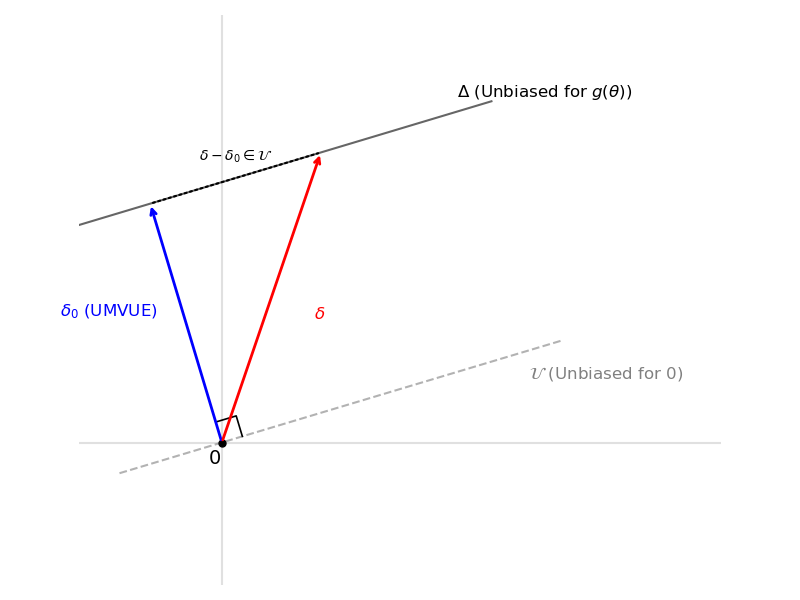
\includegraphics[width=0.8\linewidth]{umvue_theorem.png}
	\end{center}
\end{remark}

\begin{example}
	Let $X$ be a discrete random variable on $\{-1, 0, 1, 2, \dots \}$ such that $\PP(X = -1) = p$ and $\PP(X = x) = (1-p)^2 p^x$ for $x \ge 0$. Let $p \in (0, 1)$. In the homework we will show that the only functions which have a UMVUE are those of the form $g(p) = a + b(1-p)^2$ for $a, b \in \R$. 
\end{example}

\begin{example}
	Let $X \sim \text{Binom}(2, p)$. Observe that the expected value of any estimator $\delta(X)$ will be a quadratic in $p$. Namely $\E_p \delta(X) = (1-p)^2\delta(0) + 2p(1-p)\delta(1) + p^2 \delta(2)$. This implies that no unbiased estimator (and therefore no UMVUE) exists for $g(p)$ not of this form. For instance $g(p) = p^3$ has no UMVUE.
\end{example}



\newpage
\section{Lecture 5}

\subsection{Rao-Blackwell}

\begin{theorem}[Rao--Blackwell]
	Let $L(\cdot, g(\theta))$ be a convex function for each value of $\theta$. Let $T(X)$ be any sufficient statistic and $\delta(X)$ be any estimator such that $\E_\theta |\delta(X)| < \infty$ and $R(\theta, \delta) = \E_\theta L(\delta(X), g(\theta)) < \infty$. Define $h(T) = \E_\theta[\delta(X) \mid T]$. Then $R(\theta, h) \le R(\theta, \delta)$ (the inequality is strict if $L(\cdot, g(\theta))$ is strictly convex and $\delta(X)$ does not almost surely equal $h(T)$).
\end{theorem}

\begin{proof}
	This is just an application of Jensen's inequality (the conditional form). In particular, \[
		L(h(T), g(\theta)) = L(\E_\theta[\delta(X) \mid T], g(\theta)) \le \E[L(\delta(X), g(\theta)) \mid T],
	\] with the inequality being strict if the conditions in the latter part of the theorem hold. Taking expectations on both sides yields the desired result.
\end{proof}

\begin{theorem}[Lehmann--Scheff\'e]
	Let $T(X)$ be complete sufficient for $\theta$. Let $\delta(X)$ be an unbiased estimator of $g(\theta)$ with finite risk $R(\theta, \delta) = \E_\theta L(\delta(X), g(\theta))$. If $L(\cdot, g(\theta))$ is convex then $h(T) = \E_\theta[\delta(X) \mid T]$ is unbiased and is a minimizer of $R(\theta, \cdot)$ among unbiased estimators. If $L(\cdot, g(\theta))$ is strictly convex then $h(T) = \E_\theta[\delta(X) \mid T]$ is the unique minimizer of $R(\theta, \cdot)$  (uniqueness holds up to almost sure equivalence with respect to $\PP_\theta$). 
\end{theorem}

\begin{proof}
	 Let $\tilde{\delta}(X)$ be any unbiased estimator of $g(\theta)$ and define $\tilde{h}(T) = \E_\theta[\tilde{\delta}(X) \mid T]$. By the tower law $\E_\theta \tilde{h}(T) = \E_\theta \tilde{\delta}(X) = g(\theta)$ so $\tilde{h}(T)$ is still unbiased (and the same holds for $h(T)$). Then $\E_\theta[h(T) - \tilde{h}(T)] = 0$ for all $\theta$ so completeness implies that $h = \tilde{h}$ [a.s. $\PP_\theta$]. By the previous theorem if $L(\cdot, g(\theta))$ is convex then $R(\theta, \tilde{h}) \le R(\theta, \tilde{\delta})$. Since $h = \tilde{h}$ [a.s. $\PP_\theta$] we have that $R(\theta, h) \le R(\theta, \tilde{\delta})$. Hence $h(T)$ is a minimizer of $R(\theta, \cdot)$ among unbiased estimators. If $L(\cdot, g(\theta))$ is strictly convex the previous theorem implies that $R(\theta, h) < R(\theta, \tilde{\delta})$ unless $\tilde{\delta} = h(T)$ [a.s.  $\PP_\theta$]. Hence $h(T)$ is the unique minimizer.
\end{proof}

\begin{example}
	Let $X_1, \dots, X_n \sim \mathcal{N}(\mu, \sigma^2)$. A complete sufficient statistic is $(\bar{X}, \hat{\sigma})$ (the sample mean and bias-corrected sample standard deviation). Suppose we want to find a UMVUE for $p$ such that $\PP(X_1 < p) = 3/4$. In particular $p = \mu + \sigma \Phi^{-1}(3/4)$. Then an unbiased estimator of $p$ is $\delta(X) = \bar{X} + \hat{\sigma} \Phi^{-1}(3/4)$. Since this is a function of the complete sufficient statistic, the previous theorem implies that $\delta$ is a UMVUE.
\end{example}


\subsection{Cramer-Rao Lower Bound}

\begin{theorem}[Cramer-Rao]
Assume that: \begin{enumerate}[label=(\alph*)]
	\item $\Theta \subset \R$ is an open interval.
	\item $\{p_\theta : \theta \in \Theta \}$ have common support $\mathcal X$.
	\item The derivatives $p'_\theta(x)$ exist and are finite for all $x \in \mathcal X$ and $\theta \in \Theta$.
	\item The integral may be differentiated under the integral sign:
	\[
	\frac{\partial}{\partial\theta}
	\int_{\mathcal X}p_\theta(x)\,d\mu(x)
	=
	\int_{\mathcal X}
	\frac{\partial}{\partial\theta}p_\theta(x)\,d\mu(x).
	\]
	Moreover,
	\[
	I(\theta):=
	\E_\theta\!\left[
	\left(\frac{\partial}{\partial\theta}\log p_\theta(X)\right)^2
	\right]<\infty.
	\]
	This assumption implies that
	$I(\theta)=\Var_\theta(\frac{\partial}{\partial\theta}\log p_\theta(X))$.
	\item The integral may be twice differentiated under the integral sign:
	\[
	\frac{\partial^2}{\partial\theta^2}
	\int_{\mathcal X}p_\theta(x)\,d\mu(x)
	=
	\int_{\mathcal X}
	\frac{\partial^2}{\partial\theta^2}p_\theta(x)\,d\mu(x).
	\]
	This implies that
	$I(\theta)=-\E_\theta[\frac{\partial^2}{\partial\theta^2}\log p_\theta(X)]$.
	\item $T : \mathcal X \to \R$ is an unbiased estimator of $g(\theta)$, and
	\[
	\frac{\partial}{\partial\theta}
	\int_{\mathcal X}T(x)p_\theta(x)\,d\mu(x)
	=
	\int_{\mathcal X}
	T(x)\frac{\partial}{\partial\theta}p_\theta(x)\,d\mu(x).
	\]
\end{enumerate}
Then $\Var_\theta(T(X)) \geq \frac{g'(\theta)^2}{I(\theta)}$.
\end{theorem}

\begin{proof}
	Let
	\[
	V
	=
	\frac{\partial}{\partial\theta}\log p_\theta(X)
	=
	\frac{\frac{\partial}{\partial\theta}p_\theta(X)}{p_\theta(X)}.
	\]
	As noted above, the assumptions imply that $\Var_\theta(V) = I(\theta)$. Moreover, \[
		\E_\theta[V] = \int _{\mathcal X}  \frac{\partial}{\partial\theta} p_\theta(x) d\mu(x) =  \frac{\partial}{\partial\theta} \int _{\mathcal X}  p_\theta(x) d\mu(x) = \frac{\partial}{\partial\theta} 1 = 0.
	\] We also have that, \[
		\Cov_\theta(V, T) = \int_{\mathcal{X}}  \frac{\partial}{\partial\theta} p_\theta(x) T(x) d\mu(x) = \frac{\partial}{\partial\theta}  \int_{\mathcal{X}} T(x) p_\theta(x) d\mu(x) = g'(\theta).
	\] Then by Cauchy-Schwarz, \[
		 g'(\theta)^2 = \Cov_\theta(V, T)^2 \le \Var_\theta(V) \Var_\theta(T) = I(\theta) \Var_\theta(T).
	\] Rearranging gives the desired bound.
\end{proof}

\begin{remark}
Suppose that equality holds in the CRLB. Then the application of Cauchy-Schwarz must have been an equality and therefore $V$ must be linear in $T$ (barring some degenerate cases). That is \[
	 \frac{\partial}{\partial\theta} \ln p_\theta(x) = a(\theta) T(x) + b(\theta).
\] Integrating and then exponentiating implies that \[
	p_\theta(x) = e^{A(\theta) T(x) + B(\theta)} h(x).
\] An exponential family! 
\end{remark}

\begin{remark}
	While the assumptions used for the Cramer-Rao lower bound seem strong, they often hold. For example, see Lehmann and Casella~\cite[Theorem 1.5.8, p.~27]{LehmannCasella1998} for a general result about exponential families.
\end{remark}


\newpage

\section{Lecture 6}

\subsection{Cramer-Rao Lower Bound (Multi-Parameter Case)}

\begin{theorem}[Cramer-Rao]
	Assume that: \begin{enumerate}[label=(\alph*)]
		\item $\Theta \subset \R^k$ is open.
		\item $\{p_\theta : \theta \in \Theta \}$ have common support $\mathcal X$.
		\item The gradients $\nabla p_\theta(x)$ exist and are finite for all $x \in \mathcal X$ and $\theta \in \Theta$.
		\item The integral may be differentiated under the integral sign:
		\[
		\nabla_\theta\int_{\mathcal X}p_\theta(x)\,d\mu(x)
		=
		\int_{\mathcal X}\nabla_\theta p_\theta(x)\,d\mu(x).
		\]
		\item The integral may be twice differentiated under the integral sign:
		\[
		\nabla_\theta^2\int_{\mathcal X}p_\theta(x)\,d\mu(x)
		=
		\int_{\mathcal X}\nabla_\theta^2p_\theta(x)\,d\mu(x).
		\]
		\item $\delta : \mathcal X \to \R$ is an unbiased estimator of $g(\theta)$, and
		\[
		\nabla_\theta\int_{\mathcal X}\delta(x)p_\theta(x)\,d\mu(x)
		=
		\int_{\mathcal X}\delta(x)\nabla_\theta p_\theta(x)\,d\mu(x).
		\]
		\item The Fisher information matrix
		\[
		I(\theta):=\E_\theta[-\nabla_\theta^2\log p_\theta(X)]
		\]
		is finite and positive definite.
	\end{enumerate}
	Then $\Var_\theta(\delta(X)) \geq \nabla_\theta g(\theta)^\top {I^{-1}(\theta)} \nabla_\theta g(\theta)$.
\end{theorem}

\begin{proof}
Let $\psi_i(x) = \frac{\partial}{\partial\theta_i} \ln p_\theta(x)$. Then $\E \psi_i(X) = 0$ by assumption (d). Fix some $\alpha \in \R^k$ so that $\E \alpha^\top \psi = 0$ (here $\psi$ denotes the vector $(\psi_1, \dots, \psi_k)^\top)$. Then by the assumptions $\Var(\alpha^\top \psi) = \alpha^\top I(\theta) \alpha$ and $$
\Cov(\delta(X), \alpha^\top \psi) = \alpha^\top \E_\theta[\delta(X) \psi] = \alpha^\top \int_{\mathcal X} \delta(x) \nabla_\theta p_\theta(x) d\mu(x) = \alpha^\top \nabla_\theta g(\theta).
$$ Then by Cauchy-Schwarz \[
	(\alpha^\top \nabla_\theta g(\theta))^2 \leq \Var_\theta(\delta(X)) (\alpha^\top I(\theta) \alpha) \implies \sup_{\alpha} \frac{\alpha^\top \nabla_\theta g(\theta) \nabla_\theta g(\theta)^\top \alpha }{\alpha^\top I(\theta) \alpha} \le  \Var_\theta(\delta(X)).
	\] Applying the change of parameters $\alpha \leftarrow I(\theta)^{-1/2} \alpha$, the lower bound becomes
	\begin{align*}
	\Var_\theta(\delta(X))
	&\ge
	\sup_{\alpha:\|\alpha\|=1}
	\alpha^\top
	\left[
	I(\theta)^{-1/2}\nabla_\theta g(\theta)
	\nabla_\theta g(\theta)^\top I(\theta)^{-1/2}
	\right]\alpha \\
	&=
	\lambda_{\max}\!\left(
	I(\theta)^{-1/2}\nabla_\theta g(\theta)
	\nabla_\theta g(\theta)^\top I(\theta)^{-1/2}
	\right).
	\end{align*}
	Finally, using the fact that $\lambda_{\max}(AB) = \lambda_{\max}(BA)$ if $AB$ and $BA$ are PSD, we have that
	\begin{align*}
	&\lambda_{\max}\!\left(
	I(\theta)^{-1/2}\nabla_\theta g(\theta)
	\nabla_\theta g(\theta)^\top I(\theta)^{-1/2}
	\right) \\
	&\qquad=
	\lambda_{\max}\!\left(
	\nabla_\theta g(\theta)^\top I(\theta)^{-1}
	\nabla_\theta g(\theta)
	\right) \\
	&\qquad=
	\nabla_\theta g(\theta)^\top I(\theta)^{-1}
	\nabla_\theta g(\theta).
	\end{align*}
\end{proof}

\begin{remark}
For the sake of completeness here is the proof of the fact that $\lambda_{\text{max}}(AB) = \lambda_{\text{max}}(BA)$ if $AB$ and $BA$ are PSD as it is not commonly known. Note that we assume that the dimensions of $A$ and $B$ are such that $AB$ and $BA$ are well defined square matrices. Let $\lambda$ be a non-zero eigenvalue of $AB$ with corresponding eigenvector $v$. Then $ABv = \lambda v$ which implies $BABv = \lambda Bv$. Grouping terms we see that $BA(Bv) = \lambda (Bv)$. We would like to conclude that $Bv$ is an eigenvector of $BA$ with eigenvalue $\lambda$. To do this we must show that $Bv \neq 0$. But this must be the case else we would have $ABv = 0$ which violates the fact that $v$ is an eigenvector of $AB$ with a non-zero eigenvalue. Hence $\lambda$ is also an eigenvalue of $BA$. A symmetric argument implies that any non-zero eigenvalue of $BA$ is also one of $AB$. Hence $AB$ and $BA$ share the same set of non-zero eigenvalues implying that their maximum eigenvalue is the same.
\end{remark}

\begin{remark}
	The above proof can be generalized further to allow for multi-dimensional estimators $\delta: \mathcal X \to \R^d$. In this case the bound becomes $\Var_\theta(\delta(X)) \succeq dg(\theta) {I^{-1}(\theta)} dg(\theta)^\top$ where $dg(\theta)$ denotes the Jacobian matrix of $g$.
\end{remark}


\begin{example}
	Let $X_1, \dots, X_n \overset{iid}{\sim} \mathcal N(\mu, \theta)$ for $\mu \in \R$ and $\theta > 0$. This family has log-likelihood \[
		\ln p_{\mu, \theta}(x) = -\frac{n}{2} \ln(2\pi \theta) - \frac{1}{2\theta}\sum_{i=1}^n (x_i - \mu)^2 .
	\] If we treat $\theta$ as known we can compute the CRLB for $g(\mu) = \mu$ by first computing the derivatives: \[
		\frac{\partial \ln p_{\mu, \theta}(x)}{\partial \mu}(x) = \frac{1}{\theta} \sum_{i=1}^n (x_i - \mu), \quad
		\frac{\partial^2 \ln p_{\mu, \theta}(x)}{\partial \mu^2}(x) = -\frac{n}{\theta}.
	\] Then the CRLB is $\Var(\delta(X)) \ge \frac{\theta}{n}$. If $\theta$ is unknown we must also compute: \[
		\frac{\partial^2 \ln p_{\mu, \theta}(x)}{\partial \mu\partial \theta}(x) = -\frac{1}{\theta^2} \sum_{i=1}^n (x_i - \mu), \quad 
		\frac{\partial^2 \ln p_{\mu, \theta}(x)}{\partial \theta^2}(x) = \frac{n}{2\theta^2} - \frac{1}{\theta^3} \sum_{i=1}^n (x_i - \mu)^2.
	\] Taking expectations we find that the Fisher information matrix is \(
		I(\mu, \theta) = \begin{pmatrix}
		\frac{n}{\theta} & 0 \\
		0 & \frac{n}{2\theta^2}
		\end{pmatrix}.
	\) We also compute $\nabla g(\mu, \theta) = (1, 0)^\top$ where $g(\mu, \theta) = \mu$. Then the CRLB takes the form $\Var(\delta(X)) \ge (1, 0) I^{-1}(\mu, \theta) (1, 0)^\top = \frac{\theta}{n}$. The bound is unchanged because the Fisher information matrix happened to be diagonal. Such a Fisher information matrix is not common (this is a handpicked example).
\end{example}

\begin{example}
	Let $X \sim \text{Pois}(\lambda)$ for $\lambda > 0$. The log likelihood is $\ln p_\lambda(x) = -\lambda + x\ln(\lambda) - \ln(x!)$. Then the Fisher information is \[
		I(\lambda) = \E\left[-\frac{\partial^2}{\partial\lambda^2} X\ln(\lambda) - \lambda \right] = \E\left[\frac{X}{\lambda^2}\right] = \frac{1}{\lambda}.
	\] The CRLB is $\Var(\delta(X)) \ge \lambda$.
\end{example}

\noindent The following theorem characterizes how reparameterization affects the Fisher information.
\begin{theorem}
	 Let $\tau = h(\theta)$ where $h$ is invertible and differentiable. Then $I(\theta) = h'(\theta)^2 I(\tau)$.
\end{theorem}

\begin{proof}
	\begin{align*}
	I(\theta)
	&=
	\E\!\left[
	\left(\frac{\partial}{\partial\theta}\log p_\theta(X)\right)^2
	\right] =
	\E\!\left[
	\left(
	\frac{\partial\tau}{\partial\theta}
	\frac{\partial}{\partial\tau}\log p_\theta(X)
	\right)^2
	\right] \\
	&=
	\left(\frac{\partial\tau}{\partial\theta}\right)^2
	\E\!\left[
	\left(\frac{\partial}{\partial\tau}\log p_\theta(X)\right)^2
	\right] =h'(\theta)^2I(\tau).
	\end{align*}
\end{proof}

\newpage
\section{Lecture 7}

\subsection{Average Case Optimality}

Suppose $X \sim \PP_\theta$ for some $\theta \in \Theta$. So far we have thought of $\theta$ non-stochastically. We will now allow ourselves to think of $\theta$ as a random variable. In particular define a probability measure $\pi$ on $\Theta$ and think of $\theta \sim \pi$. Let $\delta(X)$ be an estimator for $g(\theta)$ where $g : \Theta \to \R$, $\delta : \mathcal X \to \R$. For each fixed $\theta$, the frequentist risk is 
\[
	R(\theta, \delta) = \E_{X \sim \PP_\theta} L(\delta(X), g(\theta)).
\]
When $\theta \sim \pi$, we can average this quantity with respect to $\theta$ to obtain the Bayes risk
\[
	r(\pi, \delta) = \E_{\theta \sim \pi} R(\theta, \delta).
\]
If an estimator $\delta_\pi$ minimizes $r(\pi, \delta)$, we call it a Bayes estimator. 

\medskip \noindent In the so-called Bayesian framework $\pi$ is usually called the prior distribution and the conditional distribution of $\theta \mid X = x$ is usually called the posterior distribution. Suppose $\PP_\theta$ has densities $p_\theta$ with respect to a $\sigma$-finite dominating measure $\mu$. Then the marginal density of $X$ is defined as $p_X(x) := \int_{\Theta} p_\theta(x) d\pi(\theta)$.

\begin{theorem}
if $L(\delta(X), g(\theta)) = (\delta(X) - g(\theta))^2$ is the squared error loss function then the posterior mean $\E[g(\theta) \mid X]$ is a Bayes estimator for $g(\theta)$.
\end{theorem}

\begin{proof}
	Let $\delta$ be an arbitrary estimator. Then 
	\begin{align*}
	\E[(\delta(X) - g(\theta))^2] &= \E[(\delta(X) - \E[g(\theta) \mid X] + \E[g(\theta) \mid X] - g(\theta))^2] \\
	&=  \E[(\delta(X) - \E[g(\theta) \mid X])^2] + \E \Var(g(\theta) \mid X) + 0.
	\end{align*}
	The expression above is uniquely minimized at $\delta(X) = \E[g(\theta) \mid X]$ (a.e. $p_X$).
\end{proof}

\begin{proposition}
	$\delta_\pi(X) = \E[g(\theta) \mid X]$ is not unbiased unless $\PP(\delta_\pi(X) = g(\theta)) = 1$.
\end{proposition}

\begin{proof}
	Suppose $\delta_\pi$ was unbiased. Then $\E[\delta_\pi(X) \mid \theta] = g(\theta)$ for all $\theta$. Then, \[
		\E[(\delta_\pi(X) - g(\theta))^2] = \E[\delta_\pi^2(X)] + \E[g^2(\theta)] - 2\E[\delta_\pi(X) g(\theta)].
	\] Since $\E[\delta_\pi(X) g(\theta)] = \E[\delta_\pi(X) \E[g(\theta) \mid X]] = \E[\delta_\pi^2(X)]$ the expression above equals \[
		\E[(\delta_\pi(X) - g(\theta))^2] = \E[g^2(\theta)] -  \E[\delta_\pi^2(X)].
	\] Moreover since $\E[\delta_\pi(X) g(\theta)] = \E[g(\theta) \E[\delta_\pi(X) \mid \theta]] = \E[g(\theta)^2]$ we also have that \[
		\E[(\delta_\pi(X) - g(\theta))^2] = \E[\delta_\pi^2(X)] - \E[g^2(\theta)].
	\] Hence \[
		\E[(\delta_\pi(X) - g(\theta))^2]  = \E[g^2(\theta)] -  \E[\delta_\pi^2(X)] = \E[\delta_\pi^2(X)] - \E[g^2(\theta)] \implies \E[(\delta_\pi(X) - g(\theta))^2]  = 0.
	\]
	So $\delta_\pi(X) = g(\theta)$ almost surely.
\end{proof}

\noindent One may ask when a Bayes estimator is unique. We have already seen that for the squared error loss the posterior mean will be the unique Bayes estimator almost surely with respect to the marginal. But when we talk about uniqueness we usually want it almost surely with respect to $\PP_\theta$ for all $\theta$. A sufficient condition for this is if the marginal dominates the conditionals $\{\PP_\theta : \theta \in \Theta \}$. When this does not hold the Bayes estimator may not be unique as demonstrated in the following example.

\begin{example}
	Let $X \sim \text{Binom}(n, \theta)$ and $\theta \sim \pi = \text{Bern}(\frac{1}{2})$. Then \[
		\PP(\theta = 1 \mid X) = \frac{\mathbf{1}[X=n]}{\mathbf{1}[X=n]+\mathbf{1}[X=0]}.
	\] Hence $\delta_\pi(0) = 0$ and $\delta_\pi(n) = 1$ and is arbitrary elsewhere. This is unique with respect to the marginal distribution but not with respect the conditionals which put probability mass on $\{0, n\}^c$.
\end{example}


\newpage
\section{Lecture 8}

\subsection{Minimaxity}

In the previous lecture we saw how summarizing the risk $R(\theta, \delta)$ as a single number allows us to discuss optimality in a sensible way. The minimax framework takes a similar approach. Instead of summarizing the risk using a prior, we consider the worst-case risk: $\sup_\theta R(\theta, \delta)$. 

\begin{definition}
	$\delta_{\text{MM}}$ is minimax (MM) if $\sup_\theta R(\theta, \delta_{\text{MM}}) = \inf_{\delta} \sup_\theta R(\theta, \delta)$. That is if it achieves the best possible worst case risk.
\end{definition}

\noindent Recall that if $\Lambda$ is a prior on $\Theta$, the Bayes risk of an estimator $\delta$ is
\[
	r(\Lambda, \delta) = \E_{\theta \sim \Lambda}[R(\theta, \delta)].
\]
A Bayes estimator $\delta_\Lambda$ is any estimator that minimizes this quantity, and we write the optimal Bayes risk as
\[
	r(\Lambda, \delta_\Lambda) = \inf_\delta r(\Lambda, \delta) =: r_\Lambda.
\]
We often have many choices for the prior $\Lambda$, yielding many different optimal Bayes risks $r_\Lambda$. The prior with the largest optimal Bayes risk is called the least favorable prior. 

\begin{definition}
	A prior distribution $\Lambda$ is least favorable (LF) if $r_\Lambda \ge r_{\Lambda'}$ for all other priors $\Lambda'$.
\end{definition}

\noindent Least favorable priors allow us to connect the Bayesian and minimax frameworks.

\begin{theorem}
Let $\Lambda$ be a prior distribution on $\Theta$ and suppose $r_\Lambda = \sup_\theta R(\theta, \delta_\Lambda)$. Then, \begin{enumerate}
	\item[(i)] $\delta_\Lambda$ is MM,
	\item[(ii)] if $\delta_\Lambda$ is unique Bayes it is also unique MM,
	\item[(iii)] $\Lambda$ is LF.

\end{enumerate}
\end{theorem}

\begin{proof}
Average risk cannot exceed worst-case risk. Indeed, \[
	r(\Lambda, \delta) = \E_{\theta \sim \Lambda}[R(\theta, \delta)] \leq \E_{\theta \sim \Lambda}[\sup_\theta R(\theta, \delta)] = \sup_\theta R(\theta, \delta).
\]
Now let $\delta$ be any estimator besides $\delta_\Lambda$. Then we have that $$\sup_\theta R(\theta, \delta_\Lambda) = r_\Lambda \leq r(\Lambda, \delta) \leq \sup_\theta R(\theta, \delta).$$ The first inequality follows from the definition of the Bayes risk.  Hence $\delta_\Lambda$ is MM. If $\delta_\Lambda$ was unique Bayes the first inequality above would be strict and we would therefore have that $\delta_\Lambda$ is unique MM. Finally let $\Lambda'$ be any other prior. Then $$
r_{\Lambda'} \leq r(\Lambda', \delta_\Lambda) \leq \sup_\theta R(\theta, \delta_\Lambda) = r_\Lambda.
$$ Hence $\Lambda$ is LF.
\end{proof}

\begin{corollary}
	If $\delta_\Lambda$ is Bayes for some $\Lambda$ and $R(\theta, \delta_\Lambda)$ is constant then $\delta_\Lambda$ is MM.
\end{corollary}

\begin{example}
	Let $X \sim \text{Binom}(n, p)$ for $p \in [0, 1]$. In one of the homeworks we computed that for the prior $\pi = \text{Beta}(a, b)$ the posterior distribution of $p \mid X$ is  $\text{Beta}(a + X, n - X + b)$. The Bayes estimator for the squared error loss is therefore $\delta_\pi(X) = \E[p \mid X] = \frac{a+X}{a + b + n}$. The risk of $\delta$ is \begin{align*}
		R(p, \delta_\pi) &= \E \left[\left(\frac{a+X}{a + b + n} - p\right)^2\right] = \frac{ \E[(X - (a+b+n)p + a)^2] }{(a + b + n)^2} \\
		&= \frac{np(1-p) + (np - (a+b+n)p + a)^2}{(a + b + n)^2} \\
		&= 	\frac{[(a+b)^2 - n]p^2 + [n- 2(a+b)a]p + a^2}{(a + b + n)^2}.
	\end{align*} To make $R(p, \delta_\pi)$ constant in $p$ we can set $(a+b)^2 - n = 0$ and $n- 2(a+b)a = 0$. Solving this system yields the solution $a = b = \sqrt{n}/2$. Hence a minimax estimator for $p$ is $\delta_{\text{MM}} = \frac{X + \sqrt{n}/2}{n + \sqrt{n}}$.
\end{example}

\begin{example}
	Let $X_1, \dots, X_n \overset{iid}{\sim} \mathcal{N}(\theta, \sigma^2)$ for $\theta \in \R$ unknown (and $\sigma^2$ known). Consider the prior $\pi = \mathcal{N}(\mu, \tau^2)$. The Bayes estimator (posterior mean) is $\delta_\pi(X) =  \frac{n/\sigma^2}{n/\sigma^2 + 1/\tau^2} \bar{X} + \frac{1/\tau^2}{n/\sigma^2 + 1/\tau^2} \mu$. As $\bar{X}$ is unbiased, it cannot be a Bayes estimator for any prior. However as $\tau^2 \to \infty$, $\delta_\pi \to \bar{X}$ pointwise. In fact one can show that as $\tau^2 \to \infty$ we have that $R(\theta, \delta_\pi) \to R(\theta, \bar{X}) = \frac{\sigma^2}{n}$ (a constant risk function). This suggests $\bar{X}$ is MM but how can we prove this? The following theorem allows us to prove such a result.
\end{example}

\begin{definition}
A sequence of priors $\{\Lambda_n\}_{n = 1}^{\infty}$ is called LF if for any prior $\Lambda$ we have that $r_\Lambda \leq \lim_{n\to\infty} r_{\Lambda_n}$.
\end{definition}

\begin{theorem}
	Suppose that, for some estimator $\delta$,
	\[
	\lim_{n\to\infty} r_{\Lambda_n}
	=
	\sup_\theta R(\theta, \delta).
	\]
	Then
	\begin{enumerate}
		\item[(i)] $\delta$ is MM,
		\item[(ii)] $\{\Lambda_n\}_{n = 1}^{\infty}$ is LF.
	\end{enumerate}
\end{theorem}

\begin{proof}
	Recall that for any prior $\Lambda$ and any estimator $\delta$, the inequality $r(\Lambda, \delta) \leq \sup_\theta R(\theta, \delta)$ always holds. Let $\delta'$ be any estimator besides $\delta$. Then \[
		\sup_\theta R(\theta, \delta) = \lim_{n\to\infty} r_{\Lambda_n} \leq \limsup_{n\to\infty} \{r(\Lambda_n, \delta')\} \leq \limsup_{n\to\infty} \{\sup_\theta R(\theta, \delta')\} = \sup_\theta R(\theta, \delta').
	\] Hence $\delta$ is MM. Now let $\Lambda$ be any prior. Then \[
		r_\Lambda \leq r(\Lambda, \delta) \leq \sup_\theta R(\theta, \delta) = \lim_{n\to\infty} r_{\Lambda_n}.
	\] Hence $\{\Lambda_n\}_{n = 1}^{\infty}$ is LF.
\end{proof}

\noindent The theorems and methods above allow us to find minimax estimators in parametric classes. Non-parametric classes can be a bit more challenging. One way of finding minimax estimators in such large classes is to pass to a smaller sub-class and lift the minimax estimator back into the original class. The following theorem makes this concrete.

\begin{theorem}
	Suppose $X \sim F$ for some distribution $F \in \mathcal F$. If $\delta$ is MM for $g(F)$ with respect to a sub-class $\mathcal F_0 \subset \mathcal F$ and if \[
		\sup_{F \in \mathcal{F}_0} R(F, \delta) = \sup_{F \in \mathcal{F}} R(F, \delta)
	\] then $\delta$ is also MM for $g(F)$ with respect to the original class $\mathcal F$.
\end{theorem}
\begin{proof}
	For any $\delta'$, \[
		\sup_{F \in \mathcal{F}} R(F, \delta) = \sup_{F \in \mathcal{F}_0} R(F, \delta) \leq \sup_{F \in \mathcal{F}_0} R(F, \delta') \leq \sup_{F \in \mathcal{F}} R(F, \delta').
	\]
\end{proof}

\begin{example} \label{ex:mm}
	Let $X_1, \dots, X_n \overset{iid}{\sim} \mathcal{N}(\mu, \sigma^2)$ for $\mu \in \R$ and $\sigma^2 \in (0, M]$ for $M > 0$. Write $\vartheta=(\mu,\sigma^2)$, so the parameter space is $\Theta = \R \times (0, M]$. For the restricted class $\Theta_0 = \R \times \{M\}$ we already showed that $\bar X$ is MM for estimating $\mu$, with risk $R(\vartheta, \bar X) = \frac{M}{n}$ under squared error loss. Then \[
		\sup_{\vartheta\in\Theta} R(\vartheta, \bar X) = \sup_{\vartheta\in\Theta} \frac{\sigma^2}{n} = \frac{M}{n} = \sup_{\vartheta\in\Theta_0} R(\vartheta, \bar X).
	\] Hence $\bar X$ is minimax by the previous theorem.
\end{example}

\begin{example}
	Let $X_1, \dots, X_n \overset{iid}{\sim} \mathcal{N}(\mu, \sigma^2)$ for $\mu \in \R$ and $\sigma^2 > 0$. Let the loss function be $L((\mu, \sigma^2), \delta) = (\delta - \mu)^2 / \sigma^2$. For the restricted class $\Theta_0 = \R \times \{1\}$ (i.e. where $\mu \in \R$ and $\sigma^2 = 1$ is fixed) we have that $\bar X$ is minimax. And for this loss function we have that \[
			\sup_{(\mu,\sigma^2)\in\Theta} R((\mu,\sigma^2), \bar X) = \sup_{(\mu,\sigma^2)\in\Theta} \frac{1}{\sigma^2} \cdot \frac{\sigma^2}{n} = \frac{1}{n} = \sup_{(\mu,\sigma^2)\in\Theta_0} R((\mu,\sigma^2), \bar X).
	\] Hence $\bar X$ is minimax by the previous theorem.
\end{example}

\begin{example}
	Let $X_1, \dots, X_n \overset{iid}{\sim} F$ where $\Var(F) \le M$. In this example the class of measures we consider (all distributions with variance at most $M$) is non-parametric. For the sub-class $\Theta_0 = \{\mathcal{N}(\mu, M) : \mu \in \R \}$ we have already proved that $\bar X$ is minimax for $\E_{Y \sim F}[Y]$ (for the squared error loss). Moreover the same proof from Example \ref{ex:mm} above shows that $\bar X$ is minimax for the original class: \[
	\sup_F R(F, \bar X) = \sup_F \frac{\Var(F)}{n} = \frac{M}{n} = \sup_{\mu} R(\mathcal{N}(\mu, M), \bar X).
	\]
\end{example}


\newpage
\section{Lecture 9}

\subsection{Admissibility} 
Admissibility is a fundamental concept in decision theory. An estimator is considered admissible if no other estimator is uniformly better across the entire parameter space.

\begin{definition}
	An estimator $\delta$ is inadmissible if there exists another estimator $\delta'$ such that:
	$$R(\theta, \delta') \le R(\theta, \delta) \quad \forall \theta \in \Theta$$
	and there exists at least one $\theta_0 \in \Theta$ such that $R(\theta_0, \delta') < R(\theta_0, \delta)$.
	An estimator is admissible if it is not inadmissible.
\end{definition}

\noindent If the loss function $L(\theta, \cdot)$ is strictly convex, the risk function uniquely identifies admissible estimators.

\begin{theorem}
	Suppose the mapping $\delta \mapsto L(\theta, \delta)$ is strictly convex. If $\delta_0$ is admissible and there exists $\delta'$ such that $R(\theta, \delta_0) = R(\theta, \delta')$ for all $\theta$, then $\delta_0 = \delta'$ a.e.
\end{theorem}

\begin{proof}
	Define a midpoint estimator $\delta^* = \frac{1}{2}(\delta_0 + \delta')$. Due to strict convexity, unless $\delta_0 = \delta'$ a.e., the risk satisfies:
	$$R(\theta, \delta^*) < \frac{1}{2}[R(\theta, \delta_0) + R(\theta, \delta')] = R(\theta, \delta_0)$$
	This inequality implies $\delta^*$ is strictly better than $\delta_0$, which contradicts the assumption that $\delta_0$ is admissible.
\end{proof}

\begin{lemma}
	Any unique Bayes estimator is admissible.
\end{lemma}

\begin{proof}
		Note that unique here means unique with respect to $\PP_\theta$ for all $\theta$. Suppose $\delta_\Lambda$ is the unique Bayes estimator under a prior $\Lambda$. If it were not admissible, there would exist an estimator $\delta'$ such that $R(\theta, \delta') \le R(\theta, \delta_\Lambda)$ for all $\theta$. This would imply that the integrated Bayes risk $r(\Lambda, \delta') \le r(\Lambda, \delta_\Lambda)$, contradicting the fact that $\delta_\Lambda$ is the unique minimizer of the Bayes risk.
\end{proof}

\begin{example}
	Let $X \sim \text{Bin}(n, p)$ for $p \in [0, 1]$. The estimator $\delta(X) = \frac{X + \sqrt{n}/2}{n + \sqrt{n}}$ is minimax for $p$ under squared error loss. Recall that $\delta(X)$ is the Bayes estimator with respect to the prior $\Lambda = \text{Beta}(\sqrt{n}/2, \sqrt{n}/2)$. Note that marginally $\PP(X = k) > 0$ for all $k \in \{0, 1, \dots, n\}$. This implies that the marginal dominates the conditionals and therefore that $\delta$ is unique Bayes. Hence $\delta$ is unique minimax (by previous theorem) and admissible (by the previous lemma). 
\end{example}


\subsection{Admissibility for the Normal Location Family}
\noindent Consider the admissibility of the linear estimators $\delta_{a,b}(X) = a\bar{X} + b$ for $X_1, \dots, X_n \overset{iid}{\sim} \mathcal{N}(\theta, \sigma^2)$ where $\sigma^2 > 0$ is known.

\begin{theorem}
	Let $Y$ be an estimator such that $E_\theta Y = \theta$ and $\text{Var}_\theta Y = \sigma^2$. The linear estimator $\delta_{a,b} = aY + b$ is inadmissible under squared error loss if any of the following hold:
	\begin{enumerate}
		\item[(i)] $a > 1$
		\item[(ii)] $a < 0$
		\item[(iii)] $a = 1, b \neq 0$
	\end{enumerate}
\end{theorem}

\begin{proof}
	For a constant $c$, write $\delta_c(X) \equiv c$. The risk of $\delta_{a,b}$ is
	\[
		R(\theta, \delta_{a,b}) = E_\theta[aY + b - \theta]^2 = a^2\sigma^2 + [(a-1)\theta + b]^2.
	\]
	\begin{enumerate}
		\item[(i)] If $a > 1$, then $R(\theta, \delta_{a,b}) \ge a^2\sigma^2 > \sigma^2 = R(\theta, Y)$. Thus $Y$ dominates $\delta_{a,b}$.
		\item[(ii)] If $a < 0$, then $R(\theta, \delta_{a,b}) > [(a-1)\theta + b]^2 = (a-1)^2(\frac{b}{1-a} - \theta)^2 > (\frac{b}{1-a} - \theta)^2 = R(\theta, \delta_{b/(1-a)})$. The constant estimator $\delta_{b/(1-a)}$ is better.
		\item[(iii)] If $a = 1, b \neq 0$, then $R(\theta, \delta_{1,b}) = \sigma^2 + b^2 > \sigma^2 = R(\theta, Y)$. $Y$ dominates $Y+b$.
	\end{enumerate}
\end{proof}

\noindent This theorem implies that  $\delta_{a,b}(X) = a\bar{X} + b$ for $X_1, \dots, X_n \overset{iid}{\sim} \mathcal N(\theta, \sigma^2)$ could only be admissible in three cases:
\begin{enumerate}
	\item[(a)] The first case is $a \in (0, 1), b \in \mathbb{R}$. Under the prior $\pi = N(\mu, \tau^2)$ we have seen that $\delta_\pi(X) =  \frac{n/\sigma^2}{n/\sigma^2 + 1/\tau^2} \bar{X} + \frac{1/\tau^2}{n/\sigma^2 + 1/\tau^2} \mu$ is a bayes estimator (in fact it is a unique bayes estimator since the marginal dominates the conditionals). It turns out one can solve the system of equations \[
		 \frac{n/\sigma^2}{n/\sigma^2 + 1/\tau^2} = a, \qquad \frac{1/\tau^2}{n/\sigma^2 + 1/\tau^2} \mu = b,
	\] yielding a map $(\mu, \tau^2) = (\mu(a, b, \sigma^2), \tau^2(a, b, \sigma^2))$. So we can choose $(\mu, \tau^2)$ so that $\delta_\pi = \delta_{a,b}$. Since $\delta_{\pi}$ is unique Bayes this implies $\delta_{a,b}$ is admissible.
	\item[(b)] The second case is $a = 1, b = 0$ (this corresponds to $\delta_{a,b}(X) = \bar{X}$). The next theorem will show that the sample mean $\bar{X}$ is admissible.
	\item[(c)] The final case is $a = 0$, $b \in \R$. That is $\delta(X) \equiv b$ for some $b \in \R$. This estimator achieves zero risk at $\theta = b$. Conversely, any estimator which achieves zero risk at $\theta = b$ must be constant almost surely. Hence the constant estimators must be admissible.
	
	
\end{enumerate}

\begin{theorem}
	Let $X_1, \dots, X_n \overset{iid}{\sim} \mathcal N(\theta, \sigma^2)$ for $\theta \in \R$ unknown (and $\sigma^2 > 0$ known). Then the sample mean $\bar{X}$ is admissible for $\theta$ under the squared error loss.
\end{theorem}

\begin{proof}[Proof (Blyth's Method)]
	
	Suppose $\bar{X}$ is inadmissible. Then there exists $\delta'$ such that $R(\theta, \delta') \le R(\theta, \bar{X}) = \frac{\sigma^2}{n}$ for all $\theta$, with strict inequality for some $\theta'$. Since $R(\theta, \delta')$ is finite, Theorem 1.5.8 of Lehmann and Casella~\cite[p.~27]{LehmannCasella1998} implies that $R(\theta, \delta')$ is continuous in $\theta$. In particular, the same theorem tells us that $\E_\theta \delta'(X)^2$ and $\E_\theta \delta'(X)$ are continuous functions of $\theta$ so $R(\theta, \delta') = \E_\theta[\delta'(X)^2] - 2\theta\E_\theta[\delta'(X)] + \theta^2$ is continuous in $\theta$ as well. Then there exists $\varepsilon > 0$ and $\theta_0 < \theta' < \theta_1$ such that $R(\theta, \delta') < \frac{\sigma^2}{n} - \varepsilon$ for all $\theta \in (\theta_0, \theta_1)$. 
	
	\medskip\noindent Now let $\Lambda_\tau = \mathcal{N}(0, \tau^2)$ and $r_{\tau} = r(\Lambda_\tau, \delta_{\Lambda_\tau}) = \frac{1}{n/\sigma^2 + 1/\tau^2}$ be the optimal Bayes risk corresponding to $\Lambda_\tau$. Then for all $\tau^2 > 0$ we have that
	\begin{align*}
		\frac{\frac{\sigma^2}{n} - r(\Lambda_\tau, \delta')}{\frac{\sigma^2}{n}  - r_{\tau}} 
		&= \frac{ \frac{1}{\sqrt{2\pi \tau^2}} \int_{-\infty}^\infty (\frac{\sigma^2}{n} - R(\theta, \delta')) e^{-\frac{\theta^2}{2\tau^2}} d\theta }{\frac{\sigma^2}{n} - \frac{1}{n/\sigma^2 + 1/\tau^2}} \\
		&= \frac{n(n\tau^2 + \sigma^2)}{ \sigma^4 \sqrt{2\pi} \tau } \int_{-\infty}^\infty \left(\tfrac{\sigma^2}{n} - R(\theta, \delta')\right) e^{-\frac{\theta^2}{2\tau^2}} d\theta \\
		&\geq \frac{n(n\tau^2 + \sigma^2)}{ \sigma^4 \sqrt{2\pi} \tau } \int_{\theta_0}^{\theta_1} \varepsilon \cdot e^{-\frac{\theta^2}{2\tau^2}} d\theta.
	\end{align*}
	Now $0 \leq \varepsilon e^{-\frac{\theta^2}{2\tau^2}} \uparrow \varepsilon$ as $\tau^2 \to \infty$. Then by MCT $\int_{\theta_0}^{\theta_1} \varepsilon \cdot e^{-\frac{\theta^2}{2\tau^2}} d\theta \uparrow \int_{\theta_0}^{\theta_1} \varepsilon d\theta = \varepsilon (\theta_1 - \theta_0)$ as $\tau^2 \to \infty$. Since $\frac{n(n\tau^2 + \sigma^2)}{ \sigma^4 \sqrt{2\pi} \tau } \to \infty$ as $\tau^2 \to \infty$ we have that \[
		\lim_{\tau^2 \to \infty} \frac{\frac{\sigma^2}{n} - r(\Lambda_\tau, \delta')}{\frac{\sigma^2}{n}  - r_{\tau}}  = \infty.
	\]
	Then there exists a $\tau^\star$ such that $\frac{\frac{\sigma^2}{n} - r(\Lambda_{\tau^\star}, \delta')}{\frac{\sigma^2}{n}  - r_{\tau^\star}} > 1 \implies r(\Lambda_{\tau^\star}, \delta') < r_{\tau^\star}$ which contradicts the definition of the optimal Bayes risk. Hence $\bar X$ is admissible.
\end{proof}

\begin{lemma}
	If an admissible estimator has constant risk, it is minimax.
\end{lemma}

\begin{proof}
	Let $\delta$ be admissible with constant risk $C$. If it were not minimax, there would exist $\delta'$ such that $\sup_\theta R(\theta, \delta') < \sup_\theta R(\theta, \delta) = C$. This implies $R(\theta, \delta') < C$ for all $\theta$, contradicting the admissibility of $\delta$.
\end{proof}

\noindent This lemma implies that in the normal setting $\bar{X}$ is minimax (which we already knew). The lemma shows how admissibility can imply minimaxity. We can also prove a theorem for the opposite direction.

\begin{theorem}
	If an estimator is unique MM then it is admissible.
\end{theorem}

\begin{proof}
	Let $\delta$ be unique MM. Suppose $\delta$ is not admissible. Then there exists another estimator $\delta'$ such that $R(\theta, \delta') \leq R(\theta, \delta)$ for all $\theta$. In particular this implies that $\sup_\theta R(\theta, \delta') \leq \sup_\theta R(\theta, \delta)$ which contradicts the fact that $\delta$ is unique MM.
\end{proof}

\noindent We mentioned above that $\bar{X}$ is unique MM in the normal setting. One way to show this is as follows. If $\bar{X}$ was not unique MM there would exist an estimator $\delta'$ such that \[
	\sup_\theta R(\theta, \delta') = \sup_\theta R(\theta, \bar{X}) = \frac{\sigma^2}{n} = R(\theta, \bar{X}).
\] This implies that for all $\theta$, \[
	R(\theta, \delta') \leq R(\theta, \bar{X}).
\] Hence the inequality above must be an equality for all $\theta$ else $\bar{X}$ would be inadmissible which we know is not true. Since the squared error loss is strictly convex, we know that the risk function uniquely identifies estimators. Hence $R(\theta, \delta') = R(\theta, \bar{X})$ for all $\theta$ implies that $\delta' = \bar{X}$ a.e. for all $\theta$.

\begin{lemma}
	Let $\Theta = [a, b]$ be a closed interval. Let the loss function $L(\theta, \delta)$ satisfy $L(\theta, \delta) = 0$ for $\delta = \theta$, $L(\theta, \delta) > 0$ for $\delta \neq \theta$, and for any fixed $\theta$ be increasing as $|\theta - \delta|$ increases. Then any estimator $\delta$ such that $P_\theta[\delta \notin [a, b]] > 0$ is inadmissible.
\end{lemma}

\begin{proof}
	Consider the truncated estimator:
	$$\delta' := \begin{cases} a, & \text{if } \delta < a \\ \delta, & \text{if } \delta \in [a, b] \\ b, & \text{if } \delta > b \end{cases}$$
	This estimator $\delta'$ dominates $\delta$ uniformly over $\Theta = [a, b]$ because it is always closer to any $\theta \in [a, b]$ than the original $\delta$ was.
\end{proof}

\begin{example}
	For $X_1, \dots, X_n \overset{iid}{\sim} \mathcal N(\theta, \sigma^2)$ where $\theta \in [a, b]$, the sample mean $\bar{X}$ is neither minimax nor admissible. The lemma above is enough to prove it is not admissible. In fact, one can show that for $\delta'$ defined as above $R(\theta, \delta') < \frac{\sigma^2}{n}$ for all $\theta \in [a, b]$. By Lehmann and Casella~\cite[Theorem 1.5.8, p.~27]{LehmannCasella1998}, $R(\theta, \delta')$ is continuous in $\theta$ and therefore \[
		\sup_{\theta \in [a, b]} R(\theta, \delta') = R(\theta_0, \delta') \text{ for some } \theta_0 \in [a, b].
	\] Hence, \[
		\sup_{\theta \in [a, b]} R(\theta, \delta') = R(\theta_0, \delta') < \tfrac{\sigma^2}{n} = \sup_{\theta \in [a, b]} R(\theta, \bar{X}).
	\] Hence $\bar{X}$ is not minimax.
\end{example}



\newpage
\section{Lecture 10}

\subsection{The James-Stein Estimator}

Consider the problem of estimating $\theta \in \R$ after observing $Z \sim \mathcal{N}(\theta, \sigma^2)$ where $\sigma^2 > 0$ is known. We have previously seen that the estimator $\hat \theta = Z$ is UMVUE, unique minimax, and admissible (later we will show that it is also the MLE). One can ask if the same holds in higher dimensions. That is for the problem of estimating $\theta \in \R^n$ after observing $Z \sim \mathcal{N}(\theta, \sigma^2 I_n)$ where $\sigma^2 > 0$ is known. Indeed $\hat \theta$ will still be UMVUE, minimax, and the MLE. Surprisingly, it turns out that $\hat \theta = Z$ is inadmissible for $n > 2$. To prove this we will show that the James-Stein estimator \[
	\hat{\theta}_{\text{JS}} = \left(1 - \frac{(n-2)\sigma^2 }{\|Z\|^2}\right) Z
\] has uniformly better risk than $\hat \theta$. The difficulty in showing this comes from trying to calculate the risk of $\hat{\theta}_{\text{JS}}$. Stein's clever idea was to find an unbiased estimator of the risk which could be used to more easily calculate the risk of $\hat{\theta}_{\text{JS}}$.

\medskip \noindent 
The model we will work with for the remainder of this lecture is $Z \sim \mathcal{N}(\theta, I_n)$ for $\theta \in \R^n$ unknown. We will work with the squared error loss function and corresponding risk function \[
	R(\theta, \hat \theta) = \E_{\theta} \|\theta - \hat \theta\|^2.
\]

\begin{lemma}
	The risk function can be expressed as \[
		R(\theta, \hat \theta) = -n + \E_\theta \|Z - \hat \theta\|^2 + 2 \sum_{i=1}^n \Cov_\theta(Z_i, \hat \theta_i).
	\]
\end{lemma}

\begin{proof}
Observe that \begin{equation}
	\|Z - \hat \theta\|^2 = \|Z - \theta + \theta - \hat \theta\|^2 = \|Z - \theta\|^2 + \|\theta - \hat \theta\|^2 + 2 \langle Z - \theta, \theta - \hat \theta \rangle. \label{eq:james_stein_expansion}
\end{equation} Since $\|Z - \theta\|^2 \sim \chi^2_n$ we have that $\E_\theta  \|Z - \theta\|^2 = n$. Since $Z - \theta$ is zero mean we also have that \[
	\E_\theta[\langle Z - \theta, \theta - \hat \theta \rangle] = \Tr (\E_\theta[(Z - \theta)(\theta - \hat \theta)^\top ]) = \Tr(\Cov_\theta(Z,  -\hat \theta)) = -\sum_{i=1}^n \Cov(Z_i, \hat \theta_i).
\] Then taking expectations on both sides of (\ref{eq:james_stein_expansion}) and re-arranging gives the desired result.	
\end{proof}

\noindent Using this lemma we can get a bit closer to constructing an unbiased estimator of the risk. All we need now is an unbiased estimator of $\Cov_\theta(Z_i, \hat \theta_i)$ since $-n + \E_\theta \|Z - \hat \theta\|^2$ can be unbiasedly estimated by $-n + \|Z - \hat \theta\|^2$. To estimate the covariance we will require Stein's famous lemma. We will start by proving the univariate version.

\begin{lemma}[Stein]
Let $Z \sim \mathcal{N}(0,1)$ and $h : \R \to \R$ be absolutely continuous. Then if $\E|h'(Z)| < \infty$ we have that $\E[Z h(Z)] = \E[h'(Z)]$.
\end{lemma}

\begin{proof} 
	 A common pseudo-proof of this result uses integration by parts:
	\begin{align*}
	\int_{-\infty}^{\infty}h'(z)\varphi(z)\,dz
	&=
	h(z)\varphi(z)\Big|_{-\infty}^{\infty}
	-
	\int_{-\infty}^{\infty}h(z)\varphi'(z)\,dz \\
	&=-\int_{-\infty}^{\infty}h(z)\varphi'(z)\,dz \\
	&=\int_{-\infty}^{\infty}h(z)z\varphi(z)\,dz.
	\end{align*}
	The last step uses the fact that the derivative of the standard normal density satisfies $\varphi'(z) = -z\varphi(z)$. The reason this is only a pseudo-proof is that one must verify
	\[
	\lim_{|z|\to\infty}h(z)\varphi(z)=0.
	\]
	This turns out to follow from the assumption $\E|h'(Z)| < \infty$. However, instead of finishing the proof in this manner we will take a more direct approach used by Stein in 1981.
	
	\medskip \noindent WLOG set $h(0) = 0$ (think about why this is valid). By Fubini we have that \begin{align*}
	\int_{0}^{\infty} h'(z) \varphi(z) \,dz &=  \int_{0}^{\infty} \int_{z}^{\infty} -\varphi'(y)h'(z) \,dy \,dz \\
	&= \int_{0}^{\infty} \int_{0}^{y} -\varphi'(y)h'(z) \,dz  \,dy \\
	&=  \int_{0}^{\infty} -\varphi'(y) h(y) \,dy = \int_{0}^{\infty} y \varphi(y) h(y) \,dy.
	\end{align*} Note that Fubini applies here because 
	\begin{align*}
	\int_0^\infty\int_z^\infty
	|\varphi'(y)h'(z)|\,dy\,dz
	&=
	\int_0^\infty\int_z^\infty
	y\varphi(y)|h'(z)|\,dy\,dz \\
	&=
	\int_0^\infty\varphi(z)|h'(z)|\,dz = \E|h'(Z)|<\infty.
	\end{align*}
	Repeating the above for $(-\infty, 0)$ and adding yields the desired result.
\end{proof}

\noindent We can now readily generalize Stein's lemma to the following case:

\begin{lemma}[Stein]
	Let $Z \sim \mathcal{N}(\theta,\sigma^2)$ and $h : \R \to \R$ be absolutely continuous. Then if $\E|h'(Z)| < \infty$ we have that $\E[(Z-\theta) h(Z)] = \sigma^2 \E[h'(Z)]$.
\end{lemma}

\begin{proof}
	Observe that $Y = (Z - \theta) / \sigma \sim \mathcal{N}(0, 1)$. Then letting $f(y) = h(\sigma y + \theta)$ we have that \[
		\E[(Z-\theta) h(Z)] = \sigma \E[Y f(Y)] = \sigma \E\left[f'(Y) \right] = \sigma^2 \E[h'(\sigma Y + \theta)] = \sigma^2 \E[h'(Z)].
	\] where the second equality follows from the version of Stein's lemma proved above.
\end{proof}

\noindent Before further generalizing Stein's lemma to the multivariate case, it is useful to discuss the concept of almost differentiability. 

\begin{definition}
	A function $h : \R^n \to \R$ is almost differentiable if there exists a function $\nabla h : \R^n \to \R^n$ such that for every $z \in \R^n$, \[
		h(x + z) - h(x) = \int_{0}^{1} z^\top \nabla h(x + tz) \, dt,
	\] for almost every $x \in \R^n$.
	
\end{definition}

\begin{remark}
	Notice that if $h$ is differentiable, its gradient would satisfy the condition on $\nabla h$. Moreover, an important implication of the definition is that if $h$ is almost differentiable, the functions $h_i(z) = h(x_1, \dots, x_{i-1}, z, x_{i+1}, \dots, x_n)$ defined by fixing all but the $i$th input to $h$ are absolutely continuous (for a.e. choice of the fixed inputs).
\end{remark}

\begin{theorem}[Multivariate Stein's Lemma]
	Let $Z \sim \mathcal{N}(0, I_n)$ and $h : \R^n \to \R$ be almost differentiable. If $\E |(\nabla h(Z))_i| < \infty$ for $i = 1, \dots, n$ then $\E[Z h(Z)] = \E[\nabla h(Z)]$.
\end{theorem}

\begin{proof}
	Fix an $i \in \{1, \dots, n\}$. Then by the univariate Stein's lemma \[
		\E[Z_i h(Z) \mid Z_{-i}] = \E\left[\frac{\partial h(Z)}{\partial Z_i} \,\Big |\, Z_{-i}\right] = \E[(\nabla h(Z))_i \mid Z_{-i}].
	\] Taking expectations on both sides yields the desired result.
\end{proof}



\newpage
\section{Lecture 11}

\subsection{The James-Stein Estimator (Continued)}

Recall that we were trying to estimate $\Cov_\theta(Z_i, \hat{\theta}_i) = \E_\theta[(Z_i-\theta_i)\hat{\theta}_i]$. By the multivariate version of Stein's lemma proved in the previous lecture, we have that \[
	\Cov_\theta(Z_i, \hat{\theta}_i) = \E_\theta\left[ \frac{\partial \hat{\theta}_i}{\partial Z_i}(Z) \right].
\] Recalling that the risk can be expressed as $R(\theta, \hat \theta) = -n + \E_\theta \|Z - \hat \theta\|^2 + 2 \sum_{i=1}^n \Cov_\theta(Z_i, \hat \theta_i)$ we can now define Stein's unbiased risk estimator (SURE): \[
	\text{SURE}(\hat{\theta}) = -n + \|Z - \hat \theta\|^2 + 2 \sum_{i=1}^n \frac{\partial \hat{\theta}_i}{\partial Z_i}(Z).
\]
The key property of SURE is that $\E_\theta[\text{SURE}(\hat{\theta})] = R(\theta, \hat{\theta})$. Let us compute SURE for the James-Stein estimator \(
\hat{\theta}_{\text{JS}} = \left(1 - \frac{n-2}{\|Z\|^2}\right) Z.
\) We start by computing the partial derivatives \[
\frac{\partial (\hat{\theta}_{\text{JS}})_i}{\partial Z_i} = \frac{\partial }{\partial Z_i} \left(1 - \frac{n-2}{\|Z\|^2}\right) Z_i = \left(1 - \frac{n-2}{\|Z\|^2}\right) + \frac{2(n-2)Z_i^2}{\|Z\|^4}.
\] Then plugging this into the definition of SURE we find that 
\begin{align*}
	\text{SURE}(\hat{\theta}_{\text{JS}}) &= -n + \frac{(n-2)^2}{\|Z\|^2} + 2n \left(1 - \frac{n-2}{\|Z\|^2}\right) + 2\sum_{i=1}^n \frac{2(n-2)Z_i^2}{\|Z\|^4} \\
	&= n + \frac{(n-2)^2}{\|Z\|^2} - \frac{2n(n-2)}{\|Z\|^2} + \frac{4(n-2)}{\|Z\|^2} \\
	&= n - \frac{(n-2)^2}{\|Z\|^2}.
\end{align*}
To make sense of this recall that the risk of the MLE is $R(\theta, Z) = n$. Then we have that \[
	R(\theta, \hat{\theta}_{\text{JS}}) = \E_\theta\left[n - \frac{(n-2)^2}{\|Z\|^2}\right] < n = R(\theta, Z).
\] This immediately implies that $\hat \theta = Z$ is inadmissible. Moreover, for $\theta = 0$ it is actually possible to compute $\E_{\theta =0}[\frac{1}{\|Z\|^2}] = \frac{1}{n-2}$. This implies \[
	R(0, \hat{\theta}_{\text{JS}}) = \E_{\theta = 0}\left[n - \frac{(n-2)^2}{\|Z\|^2}\right] = n - (n-2) = 2 \ll n.
\] So at $\theta = 0$ the risk of $\hat{\theta}_{\text{JS}}$ may be significantly smaller than that of $\hat \theta$. For $\theta$ with large norms, one can show that $\hat{\theta}_{\text{JS}}$ does not beat $\hat \theta$ by a significant margin.

\subsection{Bayesian Interpretation of the James-Stein Estimator}

The following is due to Efron in 1973. Let $\theta_i \overset{iid}{\sim}  \mathcal{N}(0, \tau^2)$ and $Z_i \mid \theta_i \sim \mathcal{N}(\theta_i, 1).$ One can show that the Bayes estimator (for the loss $L(\theta, \delta) = \|\theta - \delta\|^2$) is \[
	\E[\theta \mid Z] = \left(1 - \frac{1}{1+\tau^2}\right) Z.
\] Let us now take the \textit{Empirical Bayesian} approach. That is we will now try to estimate $\tau^2$ from the data. To do this observe that marginally $Z_i \overset{iid}{\sim} \mathcal N(0, 1 + \tau^2)$. Hence $1 + \tau^2$ can be estimated by $\frac{1}{n} \sum_{i=1}^n Z_i^2 = \frac{\|Z\|^2}{n}$.  One can even show that $\frac{n-2}{\|Z\|^2}$ is an unbiased estimator of $\frac{1}{1+\tau^2}$. Plugging this into the Bayes estimator we get the estimator \[
	\left(1 - \frac{n-2}{\|Z\|^2}\right) Z.
\] We have successfully recovered the James-Stein estimator. This demonstrates how the James-Stein estimator naturally arises from a prior belief that the components of $\theta$ are all distributed near $0$. 





\newpage

\section{Lecture 12}

\subsection{Karlin's Theorem}

Recall our discussion about the admissibility of the sample mean for the normal location family (Lecture 9). In that discussion we proved admissibility for a larger class of linear estimators of the form $a \bar{X} + b$. Karlin's theorem gives a very general sufficient condition for the admissibility of such estimators. An interesting open problem is whether this condition is also necessary for admissibility.

\begin{theorem}
	Let $p_\theta(x) = \exp(\theta T(x) - B(\theta)) h(x)$ be an exponential family whose parameter space takes the form of an open interval $\Theta = (\theta_l, \theta_u) \subseteq \R$ (note that we allow $\theta_l = -\infty$ and $\theta_u = \infty$). Let \[
		\delta_{c,d}(X) = \frac{T(X)}{1+c} + \frac{cd}{1+c}. 
	\] for $c \geq 0$ and $d \in \R$. If there exists $\theta_0 \in \Theta$ such that \[
		\int_{\theta_0}^{\theta_u} \exp({-cd\theta + cB(\theta)}) \, d\theta = \infty \quad \text{and} \quad 
		\int_{\theta_l}^{\theta_0} \exp({-cd\theta + cB(\theta)}) \, d\theta = \infty
	\] then $\delta_{c,d}$ is admissible for estimating $g(\theta) = \E_\theta[T(X)] = B'(\theta)$ with respect to the squared error loss.
\end{theorem}

\begin{example}
	Let $X \sim \text{Binom}(n, \theta)$ for $\theta \in (0, 1)$. Then \[
		p(x) = \binom{n}{x} p^x (1-p)^{n-x} = \exp\left(\frac{x}{n} \cdot n \ln\left(\frac{p}{1-p}\right) - n\ln\left(\frac{1}{1-p}\right)\right) \binom{n}{x}
	\] which is an exponential family with $T(x) = x/n$, $\theta(p) = n\ln\left(\frac{p}{1-p}\right) $, and $B(\theta) = n\ln\left(\frac{1}{1-p}\right) = n\ln(e^{\theta/n}+1)$. This implies that the natural parameter space is $\Theta = \{ \theta(p) : p \in (0, 1)\} = (-\infty, \infty)$. Then to apply Karlin's theorem we must choose a $\theta_0$ and compute the corresponding integrals. Using $\theta_0 = 0$ we try to compute \[
		\int_{0}^{\infty} \exp({-cd\theta + cB(\theta)}) \, d\theta  =
		\int_{0}^{\infty} e^{-cd\theta} (1 + e^{\theta/n})^{cn} \, d\theta.
	\] Clearly the above is infinite for $c = 0$. A similar observation shows that $\int_{-\infty}^{0} e^{-cd\theta} (1 + e^{\theta/n})^{cn} \, d\theta = \infty$ for $c = 0$. Hence Karlin's theorem implies that $\delta_{0,d} = T(X)$ is admissible for estimating $\E T(X) = p$. Moreover if $c > 0$ and $0 \le d \le 1$ we have that \[
	\int_{0}^{\infty} e^{-cd\theta} (1 + e^{\theta/n})^{cn} \, d\theta \ge \int_{0}^{\infty} e^{-cd\theta} e^{c\theta} \, d\theta = \int_{0}^{\infty} e^{c\theta(1 - d)} \, d\theta = \infty
	\] and that \[
		\int_{-\infty}^0 e^{-cd\theta} (1 + e^{\theta/n})^{cn} \, d\theta \ge \int_{-\infty}^0 e^{-cd\theta} \, d\theta = \infty.
	\] Hence by Karlin's theorem $\delta_{c,d}(X) = \frac{T(X)}{1+c} + \frac{cd}{1+c}$ is admissible for $c \ge 0$ and $0 \le d \le 1$. Equivalently, $a T(X) + b$ is admissible for $a,b \ge 0$ and $a + b \leq 1$. 
\end{example}

\noindent We now give the proof of Karlin's theorem.

\medskip \noindent A similar proof appears in Lehmann and Casella~\cite[Theorem 5.2.14, pp.~331--333]{LehmannCasella1998}.

\begin{proof}
	Let $g(\theta) = \E_\theta T(X) = B'(\theta)$. Also recall that for exponential families $\Var_\theta T(X) = B''(\theta) = I(\theta)$. Let $\delta(X)$ be an arbitrary estimator and define its bias $b_\delta(\theta) = \E[\delta(X) - g(\theta)]$. Then  \[
		\E_\theta[(\delta(X) - g(\theta))^2] = b_\delta(\theta)^2 + \Var_\theta(\delta) \geq b_\delta(\theta)^2  + \frac{(b_\delta'(\theta) + g'(\theta))^2}{I(\theta)}
	\] where the last inequality follows from the CRLB. Now suppose $\delta_{c,d}$ is inadmissible for some $c$ and $d$. Then there exists $\delta_0$ such that \[
		\E_\theta[(\delta_{c,d}(X) - g(\theta))^2] \geq \E_\theta[(\delta_0(X) - g(\theta))^2] 
	\] with the inequality being strict for at least one $\theta$. Moreover since $\delta_{c,d}$ is linear in $T(X)$ it achieves the CRLB. That is, \[
			\E_\theta[(\delta_{c,d}(X) - g(\theta))^2] = b_{c,d}(\theta)^2  + \frac{(b_{c,d}'(\theta) + g'(\theta))^2}{I(\theta)}. 
	\] Hence, \[
		b_{c,d}(\theta)^2  + \frac{(b_{c,d}'(\theta) + g'(\theta))^2}{I(\theta)} \geq b_{0}(\theta)^2  + \frac{(b_{0}'(\theta) + g'(\theta))^2}{I(\theta)}.
	\] Letting $h(\theta) = b_0(\theta) - b_{c,d}(\theta)$ the above reduces to 
	\begin{align*}
		h^2(\theta) + 2h(\theta)b_{c,d}(\theta) +  \frac{2h'(\theta)b'_{c,d}(\theta)}{I(\theta)} + \frac{2h'(\theta)g'(\theta)}{I(\theta)} + \frac{h'(\theta)^2}{I(\theta)} \leq 0
	\end{align*} 
	which implies that \[
		h^2(\theta) + 2h(\theta)b_{c,d}(\theta) +  \frac{2h'(\theta)b'_{c,d}(\theta)}{I(\theta)} + \frac{2h'(\theta)g'(\theta)}{I(\theta)} \leq 0.
	\]
	Since $b_{c,d}(\theta) = \E[\delta_{c, d}(X) - g(\theta)] = \frac{g(\theta)}{1+c} + \frac{cd}{1+c} - g(\theta) = \frac{c}{1+c} (d - g(\theta))$ and $g'(\theta) = I(\theta)$ the  inequality above can be simplified further yielding, \begin{align*}
		h^2(\theta) + \frac{2c}{1+c} h(\theta) (d - g(\theta)) + \frac{2h'(\theta)}{1+c} \leq 0.
	\end{align*}
	Now define $F(\theta) = h(\theta) e^{cd\theta - cB(\theta)}$. Then $F$ satisfies \begin{align*}
		F^2(\theta) e^{-cd\theta + cB(\theta)} + \frac{2}{1+c} F'(\theta) = e^{cd\theta - cB(\theta)} \left[h^2(\theta) + \frac{2c}{1+c} h(\theta) (d - g(\theta)) + \frac{2h'(\theta)}{1+c} \right] \leq 0.
	\end{align*} Then this implies that \[
		\frac{d}{d\theta} F(\theta)^{-1} = -\frac{F'(\theta)}{F^2(\theta)} \geq \frac{1+c}{2}  e^{-cd\theta + cB(\theta)} > 0
	\] for $\theta$ such that $F(\theta) \neq 0$. Now suppose $F(\theta_0) < 0$. Then the above implies that $F$ is decreasing so that for all $\theta \ge \theta_0$, $F(\theta) < 0$. Then \[
		- F(\theta_0)^{-1}  \geq F(\theta)^{-1} - F(\theta_0)^{-1} = \int_{\theta_0}^{\theta} -\frac{F'(\theta)}{F^2(\theta)} \, d\theta \geq \frac{1+c}{2} \int_{\theta_0}^{\theta} e^{-cd\theta + cB(\theta)} \,d\theta \to \infty 
	\] which is impossible since $F(\theta_0)$ is finite. Hence $F(\theta_0) \geq 0$. A symmetrical argument (for $\theta \to -\infty$) implies that $F(\theta_0) \le 0$. Hence $F(\theta_0) = 0$. Since this holds for every $\theta_0$ (if the integrals given in the theorem are infinite for one $\theta_0$ they must be infinite for every $\theta_0$) this implies that $F(\theta) \equiv 0$. Then $h(\theta) \equiv 0$ which implies that $b_{c,d}(\theta) = b_0(\theta)$. Returning to the start of this argument we must therefore have that
	\begin{align*}
	b_{c,d}(\theta)^2
	+\frac{(b_{c,d}'(\theta)+g'(\theta))^2}{I(\theta)}
	&=\E_\theta[(\delta_{c,d}(X)-g(\theta))^2] \\
	&=\E_\theta[(\delta_0(X)-g(\theta))^2] \\
	&=b_0(\theta)^2
	+\frac{(b_0'(\theta)+g'(\theta))^2}{I(\theta)}.
	\end{align*}
	This contradicts the fact that $\E_\theta[(\delta_{c,d}(X) - g(\theta))^2] > \E_\theta[(\delta_{0}(X) - g(\theta))^2]$ for at least one $\theta$. 
\end{proof}

\begin{example}
	Suppose $\theta_l = -\infty$ and $\theta_u = \infty$ in the statement of Karlin's theorem. Then $T(X)$ is admissible for $\E_\theta T(X)$. To see why plug in $c = 0$ to the integrals given in the theorem. They become \[
		\int_{\theta_0}^\infty 1 \, d\theta \quad \text{and} \quad \int_{-\infty}^{\theta_0} 1 \, d\theta
	\] which are always infinite. 
\end{example}



\newpage
\section{Lecture 13}

\subsection{Asymptotics}

We will work in the following setup. Let $X_1, \dots, X_n \iid \PP_\theta$ for some $\theta \in \Theta$. Assume that $\{\PP_\theta : \theta \in \Theta \}$ are probability measures on $\R$ which are dominated by some $\sigma$-finite measure $\mu$. Let $p_\theta(x) = \frac{d\PP_\theta}{d\mu}(x)$ and define the likelihood of $\theta$ given $X_1, \dots, X_n$ as \[
	L(\theta \mid X) = \prod_{i=1}^n p_\theta(X_i).
\]
The likelihood function will play a central role in the asymptotic theory. 

\begin{definition}
	Let $\delta_n(X_1, \dots, X_n)$ be an estimator for $g(\theta)$. We say $\delta_n$ is consistent if $\delta_n \overset{p}{\to} g(\theta)$ under the law $\PP_\theta^{\otimes n}$ for all $\theta \in \Theta$.
\end{definition}

\begin{example}
	Let $X_1, \dots, X_n \iid \text{Bern}(\theta)$ for $\theta \in (0, 1)$. Let $g(\theta)$ be the function defined by \[
		g(\theta) = \begin{cases}
			1 & \text{if } \theta \in \Q \\
			0 & \text{if } \theta \notin  \Q
		\end{cases}.
	\] Then there does not exst a consistent sequence of estimators for $g(\theta)$. We omit the proof as it involves some fairly obscure results from analysis.
\end{example}

\begin{definition}
	A global maximizer of the likelihood function is called an MLE (An MLE may not exist and may not be unique).
\end{definition}

\begin{lemma}
Assume  
\begin{enumerate}
	\item[(A0)] The model is identifiable: $\theta_1 \neq \theta_2 \implies \PP_{\theta_1} \neq \PP_{\theta_2}$,
	\item[(A1)]  The densities $\{p_\theta : \theta \in \Theta \}$ have common support.
\end{enumerate}	
Then for all $\theta \neq \theta_0$, $\PP^{\otimes n}_{\theta_0}(L(\theta_0 \mid X) > L(\theta \mid X)) \to 1$.
\end{lemma}

\begin{proof}
	Observe that \[
		\PP^{\otimes n}_{\theta_0}(L(\theta_0 \mid X) > L(\theta \mid X)) = 
		\PP^{\otimes n}_{\theta_0}\left(\frac{1}{n} \sum_{i=1}^n \ln\left(  \frac{p_{\theta_0}(X_i)}{p_\theta(X_i)} \right) > 0 \right).
	\] By the LLN,  $\frac{1}{n}\sum_{i=1}^n \ln\left(  \frac{p_{\theta_0}(X_i)}{p_\theta(X_i)} \right) \overset{p}{\to} \text{KL}(\PP_{\theta_0}, \PP_\theta) > 0$ (the KL is non-zero because the model is identifiable). Hence, \[
	\PP^{\otimes n}_{\theta_0}\left(\frac{1}{n} \sum_{i=1}^n \ln\left(  \frac{p_{\theta_0}(X_i)}{p_\theta(X_i)} \right) > 0 \right) \to 1. 
	\]
	Note that if $\text{KL}(\PP_{\theta_0}, \PP_\theta) = \infty$ one can show that the convergence in probability still holds (i.e. that $\frac{1}{n}\sum_{i=1}^n \ln\left(  \frac{p_{\theta_0}(X_i)}{p_\theta(X_i)} \right) \overset{p}{\to} \infty$) since $\E_{\theta_0} \left[\ln\left(  \frac{p_{\theta_0}(X)}{p_\theta(X)} \right)^- \right] \leq 1 < \infty$.
\end{proof} 

\begin{corollary}
	Suppose (A0)--(A1) hold and that $|\Theta| < \infty$. Then if $\hat{\theta}_n$ is an MLE, $\PP^{\otimes n}_{\theta_0}(\hat{\theta}_n = \theta_0) \to 1$.  
\end{corollary}

\begin{proof}
	Since $\Theta$ is finite, \[
		\PP^{\otimes n}_{\theta_0}(L(\theta_0 \mid X) \leq \max_{\theta \neq \theta_0} L(\theta \mid X)) \leq \sum_{\theta \neq \theta_0} \PP^{\otimes n}_{\theta_0}(L(\theta_0 \mid X) \leq L(\theta \mid X)) \to  \sum_{\theta \neq \theta_0}  0 = 0
	\] where the inequality follows from the union bound. Since $\hat{\theta}_n = \theta_0$ on the complement of the event considered above we have that $\PP^{\otimes n}_{\theta_0}(\hat{\theta}_n = \theta_0) \to 1$.  
\end{proof}
	
\begin{theorem}
	Suppose (A0)--(A1) hold and that
	\begin{enumerate}
		\item[(A2)$\phantom{'}$] $\theta_0$ is an interior point of $\Theta \subseteq \R$,
		\item[(A3)$'$] The function $\ln(p_\theta(x))$ is continuously differentiable in an interval about $\theta_0$ (for all $x$). 
	\end{enumerate}	
	Let $\ell_n(\theta \mid X) = \sum_{i=1}^n \ln p_\theta(X_i)$. Then the equation $\frac{\partial}{\partial \theta} \ell_n(\theta \mid X) = 0$ has a root $\hat \theta_n$ with probability tending to one such that $\hat \theta_n \overset{p}{\to} \theta_0$ with respect to the law $\PP^{\otimes n}_{\theta_0}$. 
	
\end{theorem}

\begin{proof}
	Fix $\delta > 0$ small enough so that $[\theta_0 - \delta, \theta_0 + \delta] \subset \Theta$ and $\ln(p_\theta(x))$ is continuously differentiable in this neighborhood. For $\varepsilon < \delta$ the earlier lemma implies \[
	\PP^{\otimes n}_{\theta_0}(\ell_n(\theta_0) > \max\{\ell_n(\theta_0 - \varepsilon), \ell_n(\theta_0 + \varepsilon)\}) \to 1.
	\] Let $A_n = \{\ell_n(\theta_0) > \max\{\ell_n(\theta_0 - \varepsilon), \ell_n(\theta_0 + \varepsilon)\}\}$. Then on $A_n$ there exists $\hat \theta_n(\varepsilon)$ which is a maximizer of $\ell_n |_{[\theta_0 - \varepsilon, \theta_0 + \varepsilon]}$ (i.e the restriction of $\ell_n$ to $[\theta_0 - \varepsilon, \theta_0 + \varepsilon]$) and which is not achieved at the boundary of $[\theta_0 - \varepsilon, \theta_0 + \varepsilon]$. Hence on $A_n$ we must have that $|\hat \theta_n(\varepsilon) - \theta_0| < \varepsilon$ and $\ell_n'(\hat \theta_n(\varepsilon)) = 0$. Now let $\hat \theta_n$ be the closest root of $\ell_n'(\theta)$ to $\theta_0$. The above argument implies that \[
	\PP^{\otimes n}_{\theta_0}(A_n) \leq \PP^{\otimes n}_{\theta_0}(|\hat \theta_n - \theta_0| < \varepsilon) \to 1.
	\] Hence $\hat \theta_n \overset{p}{\to} \theta_0$ with respect to the law $\PP^{\otimes n}_{\theta_0}$. 
	
	\medskip \noindent One may wonder why $\hat \theta_n$ is measurable.  To see why observe that by assumption (A3), $\ell_n'$ is continuous. Then for any closed interval $I$, the event that $\ell_n'$ has a root in $I$ is 
	\[
	R(I) := \left\{ \inf_{\theta \in I \cap \Q} |\ell_n'(\theta \mid X)| = 0 \right\},
	\] 
	which is measurable since the infimum of a countable set of measurable functions is again measurable. Let $D$ be the distance from $\theta_0$ to the closest root:
	\[
	D = \inf \{ r \in \Q^+ \mid R([\theta_0 - r, \theta_0 + r]) \text{ occurs} \} 
	\]
	Notice that this is once again an infimum over a countable set of measurable functions (i.e. those of the form $r \mathbf{1}_{R([\theta_0 - r, \theta_0 + r])} + \infty \mathbf{1}_{R([\theta_0 - r, \theta_0 + r])^c}$) so $D$ is a measurable random variable taking values in $[0, \infty]$. If $D < \infty$, continuity implies the closest root is achieved at $\theta_0 + D$ or $\theta_0 - D$. Let $E$ be the measurable event that $\theta_0 + D$ is a root, i.e., $E = \{ \ell_n'(\theta_0 + D \mid X) = 0 \}$. Then we have:
	\[
	\hat \theta_n = \begin{cases} 
		\infty & \text{if } D = \infty \\ 
		\theta_0 + D & \text{if } D < \infty \text{ and } E \text{ occurs} \\ 
		\theta_0 - D & \text{if } D < \infty \text{ and } E^c \text{ occurs}. 
	\end{cases}
	\]
	Since $\hat \theta_n$ is constructed entirely from measurable variables and events, it is measurable. Note that there are some subtleties with the decomposition above. It assumes that if there are two closest roots (i.e. a tie) $\hat \theta_n$ chooses the larger one and if there are no roots $\hat \theta_n = \infty$.
\end{proof}

\begin{remark}
Note that $\hat \theta_n$ is not an estimator. This is because there may be multiple possible roots and the correct choice depends on $\theta_0$. Also $\hat \theta_n$ may not be an MLE. 	This is because roots are not necessarily global maximizers.
\end{remark}

\begin{corollary}
	Suppose (A0)--(A2), (A3)$'$ hold and $\ell_n'$ has a unique root $\hat \theta_n$. Then $\hat \theta_n \overset{p}{\to} \theta_0$. Moreover if we assume that $\Theta$ takes the form of an interval and that $\ln(p_\theta(x))$ is everywhere continuously differentiable, we have that $\PP^{\otimes n}_{\theta_0}(\hat \theta_n = \text{MLE}) \to 1$.
\end{corollary}

\begin{proof}
	The fact that $\hat \theta_n \overset{p}{\to} \theta_0$ is immediate from the previous theorem. For the second part, suppose that $\hat \theta_n$ is not a global maximizer (with probability converging to $1$). From the proof of the previous theorem, we know that $\hat \theta_n$ will be a local maximum of $\ell_n$ in an $\varepsilon$-neighborhood of $\theta_0$ (with probability converging to $1$). Since we assumed $\hat \theta_n$ is not a global maximizer, this implies there exists a local minimum between $\hat \theta_n$  and the true global maximizer. This would imply the existence of a second root which is a contradiction. Hence we must have $\PP^{\otimes n}_{\theta_0}(\hat \theta_n = \text{MLE}) \to 1$. 
	
	\medskip \noindent Note that we cannot drop the assumption that $\Theta$ is an interval for the latter result. A proof can be found \href{https://danieletaat.github.io/posts/2025/11/inconsistent_mle/}{here}.
\end{proof}



\newpage
\section{Lecture 14}

\subsection{Asymptotics (Continued)}

In this lecture we will slightly strengthen assumption (A3)$'$ from the previous lecture. In particular we will prove the following theorem.

\begin{theorem}
Suppose that (A0)--(A2) hold and that \begin{enumerate}
	\item[(A3)] $\ln(p_\theta(x))$ is three times differentiable in an interval about $\theta_0$ (for all $x$) and there exists a $\delta > 0$ and a function $M_{\theta_0}(x)$ such that for all $\theta \in (\theta_0 - \delta, \theta_0 + \delta)$, \[
		\left| \frac{\partial^3}{\partial \theta^3} \ln p_\theta(x) \right| \leq M_{\theta_0}(x)
	\] with $\E_{\theta_0} M_{\theta_0}(X) < \infty$,
	\item[(A4)$\phantom{'}$] $\int p_\theta(x) d\mu(x)$ can be twice differentiated under the integral sign and the first and second order definitions of the Fisher information agree and satisfy $0 < I(\theta_0) < \infty$.
\end{enumerate}
Then any consistent sequence of roots $\hat \theta_n$ of $\ell_n'(\theta \mid X)$  satisfies, \[
	\sqrt{n}(\hat \theta_n - \theta_0) \overset{d}{\to} \mathcal{N}(0, I(\theta_0)^{-1})
\]
\end{theorem}

\begin{proof}
	Define the event $A_n = \{ |\hat \theta_n - \theta_0| < \delta \}$. Since $\hat \theta_n$ is consistent we have that $\PP(A_n) \to 1$ as $n \to \infty$. Place ourselves on this event. By Taylor's theorem we have that \[
		\ell_n'(\hat \theta_n) = 0 = \ell'_n(\theta_0) + (\hat \theta_n - \theta_0) \ell_n''(\theta_0) + \frac{(\hat \theta_n - \theta_0)^2}{2} \ell_n'''(\xi_n)
	\] for some $\xi_n$ between $\theta_0$ and $\hat \theta_n$. Moreover on $A_n$ we have that, \[
		\left| \frac{\ell_n'''(\xi_n)}{n}\right| = \left| \frac{1}{n} \sum_{i=1}^n \left[ \frac{\partial^3}{\partial \theta^3} \ln p_\theta(X_i) \right]_{\theta = \xi_n} \right| \leq \frac{1}{n} \sum_{i=1}^n M_{\theta_0}(X_i) \overset{p}{\to} \E_{\theta_0} M_{\theta_0}(X) < \infty.
	\] Hence $\frac{\ell_n'''(\xi_n)}{n} = O_p(1)$ which implies that \begin{align*}
		0 = \frac{1}{n}\ell'_n(\theta_0) + (\hat \theta_n - \theta_0) \frac{\ell_n''(\theta_0)}{n}  + \frac{(\hat \theta_n - \theta_0)^2}{2} O_p(1) \implies  
		\sqrt{n}(\hat \theta_n - \theta_0) = \frac{-\frac{1}{\sqrt{n}} \ell'_n(\theta_0)}{\frac{\ell_n''(\theta_0)}{n}  + \frac{(\hat \theta_n - \theta_0)}{2} O_p(1)}.
	\end{align*}
	Since $\hat \theta_n$ is consistent we have that $(\hat \theta_n - \theta_0) = o_p(1)$ and therefore that the term $\frac{(\hat \theta_n - \theta_0)}{2} O_p(1)$ in the denominator above is also $o_p(1)$. Moreover the LLN implies that $\frac{\ell_n''(\theta_0)}{n} \overset{p}{\to} -I(\theta_0)$ and the CLT implies that $\frac{1}{\sqrt{n}} \ell'_n(\theta_0) \overset{d}{\to} \mathcal N(0, I(\theta_0))$. Then by Slutsky's theorem we have that \[
		\sqrt{n}(\hat \theta_n - \theta_0) \overset{d}{\to} \mathcal{N}(0, I(\theta_0)) \cdot \frac{1}{I(\theta_0)} = \mathcal{N}(0, I(\theta_0)^{-1}).
	\] 
\end{proof}

\begin{remark}
	The CRLB gives $\Var_{\theta} (\hat \theta_n) \geq \frac{(\frac{\partial}{\partial \theta} \E_\theta \hat \theta_n (X))^2}{n I(\theta)}$. Suppose that $\E_\theta \hat \theta_n (X) \approx \theta$. Then the CRLB gives $\Var_{\theta} (\hat \theta_n) \gtrsim \frac{1}{nI(\theta)}$ which implies that $\Var_{\theta} (\sqrt{n}(\hat \theta_n - \theta)) \gtrsim \frac{1}{I(\theta)}$.
\end{remark}

\begin{definition}
	We say an estimator $\hat \theta_n$ is asymptotically efficient if $\sqrt{n}(\hat \theta_n - \theta_0) \overset{d}{\to} \mathcal{N}(0, I(\theta_0)^{-1})$ for all $\theta_0 \in \Theta$. 
\end{definition}

\begin{example}
	Let $X_1, \dots, X_n \overset{iid}{\sim} \mathcal{N}(\theta_0, 1)$ and $\Theta = \R$. The MLE in this model is $\bar X$ and it is easy to verify that \[
		\sqrt{n}(\bar X - \theta_0) \sim \mathcal N(0, 1).
	\] One can also check that $I(\theta) \equiv 1$. Hence the MLE is asymptotically efficient (in fact it is efficient in finite samples).
\end{example}

\noindent Asymptotic efficiency is not necessarily the best measure of an estimator's optimality. Consider the following example due to Hodges.

\begin{example}[Hodges' Estimator]
	Let $X_1, \dots, X_n \overset{iid}{\sim} \mathcal{N}(\theta_0, 1)$ and define the estimator $$
	\delta_n(X) = \begin{cases}
		\bar X & \text{if } |\bar X| > n^{-\frac{1}{4}}, \\
		0 & \text{if } |\bar X| \leq n^{-\frac{1}{4}}.
	\end{cases}
	$$ 
	Let $Z_n=\sqrt n(\bar X-\theta_0)\sim\mathcal N(0,1)$. Then
	\begin{align*}
	\PP_{\theta_0}(|\bar X|\le n^{-1/4})
	&=
	\PP_{\theta_0}\!\left(
	-n^{1/4}-\sqrt n\,\theta_0
	<Z_n<
	n^{1/4}-\sqrt n\,\theta_0
	\right) \\
	&=
	\Phi(n^{1/4}-\sqrt n\,\theta_0)
	-
	\Phi(-n^{1/4}-\sqrt n\,\theta_0).
	\end{align*}
	If $\theta_0 > 0$ the expression above converges to $\Phi(-\infty) - \Phi(-\infty) = 0 - 0 = 0$. If $\theta_0 < 0$ the expression converges to $\Phi(\infty) - \Phi(\infty) = 1 - 1 = 0$. If $\theta_0 = 0$ the expression converges to $\Phi(\infty) - \Phi(-\infty) = 1 - 0 = 1$. Hence for $\theta_0 \neq 0$, $\delta_n(X) = \bar X$ with probability converging to $1$ and for $\theta_0 = 0$, $\delta_n(X) = 0$ with probability converging to $1$. Then it is not hard to see that \begin{align*}
		&\sqrt{n} (\delta_n(X) - \theta_0) \overset{d}{\to} \mathcal{N}(0,1) \quad \text{if } \theta_0 \neq 0 \\
		&\sqrt{n} (\delta_n(X) - \theta_0) \overset{d}{\to} \mathcal{N}(0,0) \quad \text{if } \theta_0 = 0.
	\end{align*}
	Hence Hodges' estimator has strictly better asymptotic variance than the MLE (albeit only at $\theta_0 = 0$). However this does not capture the whole story. Intuitively Hodges' estimator is sacrificing performance near $\theta_0 = 0$ in exchange for better performance at $\theta_0 = 0$. One can perform a local asymptotic analysis (LAA) to see this more clearly. A more informal way to see this is to compare the $\sup$ risks of the estimators. For the MLE we get that \[
		\sup_{\theta \in \R} \E_{\theta} (\bar X - \theta)^2 = \frac{1}{n}
	\] while for Hodges' estimator we get that \[
		\sup_{\theta \in \R} \E_{\theta} (\delta_n(X) - \theta)^2 \geq \E_{\theta = n^{-1/4}} (\delta_n(X) - n^{-1/4})^2 \geq (n^{-1/4})^2 \PP_{\theta = n^{-1/4}}(|\bar X| \leq n^{-\frac{1}{4}}) \sim \frac{1}{2\sqrt{n}}.
	\] Since $\frac{1}{n} \ll \frac{1}{2\sqrt{n}}$ we see that Hodges' estimator has worse $\sup$ risk.
\end{example}





\section{Lecture 15}

\subsection{Le Cam's Theorem and Newton-Raphson Update}

\begin{theorem}[Le Cam's Theorem]
	Suppose assumptions (A0)--(A2), (A4) hold and
	\begin{enumerate}
		\item[(A3)$''$] $p_\theta(x)$ is twice differentiable in a neighborhood of $\theta_0$, and there exists a $\delta > 0$ and a function $M_{\theta_0}(x)$ such that 
		\[
		\sup_{\theta : |\theta - \theta_0| < \delta} \left| \frac{\partial^2}{\partial \theta^2} \ln p_\theta(x) \right| \leq M_{\theta_0}(x)
		\] 
		and $\E_{\theta_0} M_{\theta_0}(X) < \infty$.
	\end{enumerate}
	Suppose that $\delta_n$ is an estimator satisfying \[
		\sqrt{n}(\delta_n(X) - \theta_0) \overset{d}{\to} \mathcal{N}(0, \nu(\theta_0))
	\] for all $\theta_0 \in \Theta$. Then the set $\{\theta \in \Theta : \nu(\theta) < I(\theta)^{-1} \}$ has Lebesgue measure 0.
\end{theorem}

\begin{proof} The proof will be given next semester.
\end{proof}

\begin{remark}
	Assumptions (A0)--(A4) hold for most one-parameter exponential families. For example to verify (A3) notice that if $p_\theta(x) = e^{T(x)\theta - B(\theta)} h(x)$, then $\frac{\partial^3}{\partial \theta^3} \ln p_\theta(x) = -B'''(\theta)$, which is bounded on compact sets.
\end{remark}

\noindent Suppose you want to solve for $\theta$ such that $g(\theta) = 0$ given an initial guess $\theta_0$. Suppose $g(\theta_1) = 0$. Then \[
	g(\theta_1) = 0 \approx g(\theta_0) + g'(\theta_0) (\theta_1 - \theta_0) \implies \theta_1 \approx \theta_0 - \frac{g(\theta_0)}{g'(\theta_0)}
\]
This gives rise to the Newton-Raphson update step: $\theta_1 = \theta_0 - \frac{g(\theta_0)}{g'(\theta_0)}$.

\begin{theorem}
	Assume (A0)--(A4) hold. Let $\tilde{\theta}_n$ be a $\sqrt{n}$-consistent estimator under $\PP_{\theta_0}$, i.e., $\sqrt{n}(\tilde{\theta}_n - \theta_0) = O_p(1)$. Define $\delta_n = \tilde{\theta}_n - \frac{\ell_n'(\tilde{\theta}_n)}{\ell_n''(\tilde{\theta}_n)}$. Then, 
	\[
	\sqrt{n}(\delta_n - \theta_0) \overset{d}{\to} \mathcal{N}(0, I(\theta_0)^{-1})
	\] 
\end{theorem}

\begin{proof}
	By Taylor's theorem we have 
	\[
	\ell_n'(\tilde{\theta}_n) = \ell_n'(\theta_0) + (\tilde{\theta}_n - \theta_0) \ell_n''(\theta_0) + \frac{(\tilde{\theta}_n - \theta_0)^2}{2} \ell_n'''(\xi_n)
	\]
	Substituting this into the definition of $\delta_n$ yields the following expanded form:
	\begin{align*}
		\delta_n = \tilde{\theta}_n - \frac{\ell_n'(\theta_0) + (\tilde{\theta}_n - \theta_0) \ell_n''(\theta_0) + \frac{(\tilde{\theta}_n - \theta_0)^2}{2} \ell_n'''(\xi_n)}{\ell_n''(\tilde{\theta}_n)} \\
	\end{align*}
	which implies that \begin{align}
		\sqrt{n}(\delta_n - \theta_0) &= \sqrt{n} (\tilde{\theta}_n - \theta_0) - \frac{ \sqrt{n} \ell_n'(\theta_0)}{\ell_n''(\tilde{\theta}_n)} - \frac{\sqrt{n}  (\tilde{\theta}_n - \theta_0) \ell_n''(\theta_0) }{\ell_n''(\tilde{\theta}_n)}
		- \frac{\sqrt{n}  (\tilde{\theta}_n - \theta_0)^2 \ell_n'''(\xi_n) }{2\ell_n''(\tilde{\theta}_n)} \nonumber \\
		&= 
		-\frac{ \frac{1}{\sqrt{n}} \ell_n'(\theta_0)}{\frac{1}{n} \ell_n''(\tilde{\theta}_n) } 
		+ \sqrt{n} (\tilde{\theta}_n - \theta_0) \left[ 1 - \frac{\ell_n''(\theta_0) }{\ell_n''(\tilde{\theta}_n)}
		- \frac{(\tilde{\theta}_n - \theta_0) \ell_n'''(\xi_n) }{2\ell_n''(\tilde{\theta}_n)} \right] \label{eq:nr_expansion}
	\end{align}
	Now by Taylor's theorem we have that \[
		\frac{1}{n}\ell_n''(\tilde{\theta}_n) = \frac{1}{n}\ell_n''(\theta_0) + (\tilde{\theta}_n - \theta_0) \frac{1}{n} \ell_n'''(\xi'_n).
	\]
	Since $ \frac{1}{n}\ell_n''(\theta_0) \overset{p}{\to} -I(\theta_0)$, $(\tilde{\theta}_n - \theta_0) = o_p(1)$, and $\frac{1}{n} \ell_n'''(\xi'_n) = O_p(1)$, Slutsky's theorem implies that $\frac{1}{n}\ell_n''(\tilde{\theta}_n) \overset{p}{\to} -I(\theta_0)$.  Moreover the CLT implies that $\frac{1}{\sqrt{n}} \ell'_n(\theta_0) \overset{d}{\to} \mathcal N(0, I(\theta_0))$. Then another application of Slutsky's implies that the first term in (\ref{eq:nr_expansion}) converges to $\mathcal{N}(0, I(\theta_0)^{-1})$ in distribution. Since we already know that $\sqrt{n} (\tilde{\theta}_n - \theta_0) = O_p(1)$ we need only show that \[
		1 - \frac{\ell_n''(\theta_0) }{\ell_n''(\tilde{\theta}_n)}
		- \frac{(\tilde{\theta}_n - \theta_0) \ell_n'''(\xi_n) }{2\ell_n''(\tilde{\theta}_n)} = o_p(1).
	\] Since both $\frac{1}{n}\ell_n''(\theta_0) \overset{p}{\to} -I(\theta_0)$ and $\frac{1}{n}\ell_n''(\tilde{\theta}_n) \overset{p}{\to} -I(\theta_0)$ it is clear that $\frac{\ell_n''(\theta_0) }{\ell_n''(\tilde{\theta}_n)} \overset{p}{\to} 1$. We also have that $\frac{(\tilde{\theta}_n - \theta_0) \ell_n'''(\xi_n) }{2\ell_n''(\tilde{\theta}_n)} = \frac{(\tilde{\theta}_n - \theta_0) \, \cdot \, \frac{1}{n}\ell_n'''(\xi_n) }{\frac{2}{n}\ell_n''(\tilde{\theta}_n)} = \frac{o_p(1) \, \cdot \, O_p(1)}{O_p(1)} = o_p(1)$. Hence \[
		1 - \frac{\ell_n''(\theta_0) }{\ell_n''(\tilde{\theta}_n)}
		- \frac{(\tilde{\theta}_n - \theta_0) \ell_n'''(\xi_n) }{2\ell_n''(\tilde{\theta}_n)} = 1 - (1 + o_p(1)) - o_p(1) = o_p(1)
	\] as desired.
\end{proof}

\begin{example}
	Suppose $X_1, \dots, X_n \iid \text{Cauchy}(\theta)$. One can easily verify that (A0)--(A4) hold for the Cauchy location family. The next theorem will further imply that the sample median is a $\sqrt{n}$-consistent estimator for $\theta$. Then the Newton-Raphson update of the sample median will produce an asymptotically efficient estimator.
\end{example}


\begin{theorem}[Quantile CLT]
	Suppose $X_1, \dots, X_n$ are i.i.d. random variables with distribution function $F(x)$ which is differentiable at $\theta$ with $F'(\theta) = f(\theta) \in (0, \infty)$. Setting $p = F(\theta)$ we have that \[
		\sqrt{n} (X_{(\lceil np \rceil)} - \theta) \overset{d}{\to} \mathcal{N}\left(0, \frac{p(1-p)}{f(\theta)^2}\right)
	\]
\end{theorem}

\begin{proof}
	Note that the assumptions of the theorem imply $p \in (0, 1)$. The key idea in this proof is that the following events are equivalent: \[
		\{ X_{(\lceil np \rceil)} \leq t \} \iff \left\{ \sum_{i=1}^n \mathbf{1}[X_i \leq t] \geq \lceil np \rceil \right\}.
	\] Given this fact we have that \[
		\PP(\sqrt{n} (X_{(\lceil np \rceil)} - \theta) \leq t) = \PP\left(X_{(\lceil np \rceil)} \leq \tfrac{t}{\sqrt{n}} + \theta\right) = \PP\left( \sum_{i=1}^n \mathbf{1}\left[X_i \leq \tfrac{t}{\sqrt{n}} + \theta\right] \geq \lceil np \rceil \right).
	\] Let $S_n = \sum_{i=1}^n \mathbf{1}\left[X_i \leq \tfrac{t}{\sqrt{n}} + \theta\right]$ and observe that $S_n \sim \text{Binom}\left(n, p_n\right)$ where $p_n = F(\tfrac{t}{\sqrt{n}} + \theta)$. Then \begin{equation}
		\PP(\sqrt{n} (X_{(\lceil np \rceil)} - \theta) \leq t) = \PP(S_n \geq \lceil np \rceil) = \PP\left( \frac{S_n - np_n}{\sqrt{np_n(1-p_n)}} \geq \frac{\lceil np \rceil - np_n}{\sqrt{np_n(1-p_n)}}  \right). \label{eq:quantile_clt_eq1}
	\end{equation}
	Since $F$ is continuous at $\theta$ we have that $p_n \to F(\theta) = p$ as $n \to \infty$. Then the Berry--Esseen theorem~\cite{Berry1941,Esseen1942} implies that \[
		\sup_{t \in \R} \left| \PP\left( \frac{S_n - np_n}{\sqrt{np_n(1-p_n)}} \geq t \right) - \Phi(-t) \right| \leq \frac{C}{\sqrt{n}} \left[\frac{p_n^3(1-p_n) + p_n(1-p_n)^3}{\sqrt{p_n(1-p_n)}^3} \right] \to 0.
	\] In particular this implies that \begin{equation}
	\left| \PP\left( \frac{S_n - np_n}{\sqrt{np_n(1-p_n)}} \geq \frac{\lceil np \rceil - np_n}{\sqrt{np_n(1-p_n)}}  \right) - \Phi\left( \frac{np_n - \lceil np \rceil}{\sqrt{np_n(1-p_n)}}  \right) \right| \to 0. \label{eq:quantile_clt_eq2}
	\end{equation} Moreover observe that by the definition of the derivative\[
		\frac{p_n - p}{t / \sqrt{n}} = \frac{F\left(\theta + \tfrac{t}{\sqrt{n}}\right) - F(\theta)}{t/\sqrt{n}} \to f(\theta) \implies \sqrt{n} (p_n - p) \to tf(\theta).
	\] for $t \neq 0$ and for $t = 0$ we have $\sqrt{n} (p_n - p) = 0 = tf(\theta)$. Hence \[
		\frac{np_n - \lceil np \rceil}{\sqrt{np_n(1-p_n)}} = 
		\frac{\sqrt{n}(p_n - p) + \sqrt{n}(p - \tfrac{\lceil np \rceil}{n})}{\sqrt{p_n(1-p_n)}} \to \frac{tf(\theta) + 0}{\sqrt{p(1-p)}}.
	\] Then by the continuity of $\Phi$ we have that \[
		\Phi\left( \frac{np_n - \lceil np \rceil}{\sqrt{np_n(1-p_n)}}\right) \to \Phi\left( \frac{tf(\theta)}{\sqrt{p(1-p)}} \right)
	\] Combining this with equations (\ref{eq:quantile_clt_eq1}) and (\ref{eq:quantile_clt_eq2}) we have that \[
		\PP(\sqrt{n} (X_{(\lceil np \rceil)} - \theta) \leq t) \to \Phi\left( \frac{tf(\theta)}{\sqrt{p(1-p)}} \right)
	\] which directly implies the conclusion of the theorem.
\end{proof}

\begin{remark}
	A somewhat related and useful result, P\'olya's theorem~\cite{Polya1920}, states that if $X_n \overset{d}{\to} X$ and $F_X$ is continuous, then $F_{X_n} \to F_X$ uniformly. 
\end{remark}




\newpage
\section{Lecture 16}

\subsection{Delta Method}

\begin{remark}
	Suppose an estimator $\hat \theta$ is an MLE for $\theta$. Then for any function $g(\theta)$ we may ask whether the estimator $g(\hat{\theta})$ is an MLE for $g(\theta)$. To do so we must properly define the likelihood with respect to $g(\theta)$. This is trivial if $g$ is one-to-one. If $g$ is not one-to-one things are less clear. To resolve any ambiguity we define the profile likelihood as \[
	L_g(\gamma) = \sup_{\theta: g(\theta)=\gamma} L(\theta \mid X).
	\] With this convention $g(\hat{\theta})$ will indeed be an MLE for $g(\theta)$ (i.e. $g(\hat{\theta})$ will be a global maximizer of the profile likelihood above).
\end{remark}

\begin{example}
	Suppose $X_1, \dots, X_n \iid \mathcal N(\theta, 1)$ and $g(\theta) = \theta^2$. Then the profile likelihood takes the form \[
		L_g(\gamma) = (2\pi)^{-\frac{n}{2}} e^{-\frac{1}{2} \sum_{i=1}^n X_i^2} e^{-\frac{n\gamma}{2}} \max\left\{ e^{\sqrt{\gamma} \sum_{i=1}^n X_i}, e^{-\sqrt{\gamma} \sum_{i=1}^n X_i} \right\}.
	\] 
\end{example}

\begin{example} \label{ex:poisson_exp_mle}
	Suppose $X_1, \dots, X_n \overset{iid}{\sim} \text{Pois}(\lambda)$ and we want to estimate $g(\lambda) = e^{-\lambda}$. We already know that the MLE and UMVUE for $\lambda$ is $\bar X$. Then the MLE for $g(\lambda)$ is $e^{-\bar{X}}$. However one can show that the UMVUE is given by $\left(1 - \frac{1}{n}\right)^{\sum_{i=1}^n X_i}$.
\end{example}

\begin{theorem}[Delta Method]
	Suppose $\sqrt{n}(X_n - \mu) \overset{d}{\to} \mathcal{N}(0, \sigma^2)$. If $g$ is differentiable at $\mu$, then \[
	\sqrt{n}(g(X_n) - g(\mu)) \overset{d}{\to} \mathcal{N}(0, [g'(\mu)]^2 \sigma^2).
	\]
\end{theorem}

\begin{proof}
	By Taylor's theorem, we have that \[
	g(x) = g(\mu) + (x - \mu)g'(\mu) + (x - \mu)r(x)
	\] where $r(x) \to 0$ as $x \to \mu$. Given $\varepsilon > 0$, there exists $\delta > 0$ such that $|x - \mu| < \delta \implies |r(x)| < \varepsilon$. We can write \[
	\sqrt{n}(g(X_n) - g(\mu)) = \sqrt{n}(X_n - \mu)g'(\mu) + \sqrt{n}(X_n - \mu)r(X_n).
	\] We know the first term $\sqrt{n}(X_n - \mu)g'(\mu) \overset{d}{\to} \mathcal{N}(0, [g'(\mu)]^2 \sigma^2)$. Then it suffices to show that $r(X_n) \overset{p}{\to} 0$. Because $X_n$ is consistent, we have that $\PP(|X_n - \mu| < \delta) \to 1$ which implies that $\PP(|r(X_n)| < \varepsilon) \to 1$. Since this holds for all $\varepsilon > 0$ we have that $r(X_n) \overset{p}{\to} 0$.
\end{proof}

\begin{theorem}[Second-Order Delta Method]
	Suppose $\sqrt{n}(X_n - \mu) \overset{d}{\to} \mathcal{N}(0, \sigma^2)$. If $g$ is twice differentiable at $\mu$ with $g'(\mu) = 0$. Then \[
	n(g(X_n) - g(\mu)) \overset{d}{\to} \frac{1}{2} g''(\mu) \sigma^2 \chi^2_1.
	\]
\end{theorem}

\begin{proof}
By Taylor's theorem (and the fact that $g'(\mu) = 0$) we have that \[
g(x) = g(\mu) + \frac{g''(\mu)}{2}(x - \mu)^2  + r(x) (x - \mu)^2  
\] where $r(x) \to 0$ as $x \to \mu$. Hence \[
	n(g(X_n) - g(\mu)) = \frac{g''(\mu)}{2} (\sqrt{n}(X_n - \mu))^2 + r(X_n) (\sqrt{n}(X_n - \mu))^2.
\] By the continuous mapping theorem $\frac{g''(\mu)}{2} (\sqrt{n}(X_n - \mu))^2 \overset{d}{\to}  \frac{1}{2} g''(\mu) \sigma^2 \chi^2_1$. Then it suffices to show that $r(X_n) = o_p(1)$. But this follows from same reasoning as in the previous theorem.
\end{proof}

\begin{remark}
	The Delta method can be generalized further. If we only assume that $\sqrt{n} (X_n - \mu) \overset{d}{\to} Y$ for some arbitrary random variable $Y$ the conclusion becomes\\ $\sqrt{n}(g(X_n) - g(\mu)) \overset{d}{\to} g'(\mu) Y$. A similar generalization can be made for the second order Delta method.
\end{remark}

\begin{example}
	Continuing Example \ref{ex:poisson_exp_mle} where $X_1, \dots, X_n \overset{iid}{\sim} \text{Pois}(\lambda)$ and $g(\lambda) = e^{-\lambda}$, the CLT implies that \[
		\sqrt{n} (\bar X - \lambda) \overset{d}{\to} \mathcal{N}(0, \lambda).
	\] Then the Delta method implies that \[
		\sqrt{n} (e^{-\bar X} - e^{-\lambda}) \overset{d}{\to} \mathcal{N}(0, \lambda e^{-2\lambda}).
	\]
\end{example}

\begin{example}
	Let $X_1, \dots, X_n \overset{iid}{\sim} \mathcal{N}(\theta, \sigma^2)$. Define the following estimators:
	\begin{itemize}
		\item $\delta_1(X) = \bar{X}^2$, which is the MLE.
		\item $\delta_2(X) = \bar{X}^2 - \frac{\sigma^2}{n}$, which is the UMVUE if $\sigma^2$ is known.
		\item $\delta_3(X) = \bar{X}^2 - \frac{S^2}{n}$, which is the UMVUE if $\sigma^2$ is unknown.
	\end{itemize}
	By the Delta Method, $\sqrt{n}(\delta_1(X) - \theta^2) \overset{d}{\to} \mathcal{N}(0, 4\theta^2\sigma^2)$. Since $\frac{\sigma^2}{n} = O_p(\frac{1}{n})$ and $\frac{S^2}{n} = O_p(\frac{1}{n})$, the exact same asymptotic distribution holds for $\delta_2$ and $\delta_3$.
\end{example}

\begin{example}
	Let $X_1, \dots, X_n \overset{iid}{\sim} U(0, \theta)$ for $\theta > 0$, and we want to estimate $\theta$. The estimator $X_{(n)}$ is the MLE, and $\frac{n+1}{n}X_{(n)}$ is the UMVUE. For $t \ge 0$ we have that \begin{align*}
		\PP(n(\theta - X_{(n)}) \geq t) &= \PP\left(X_{(n)} \leq \theta - \frac{t}{n}\right) \\
		&= \left(1 - \frac{t}{n\theta}\right)^n \to e^{-t/\theta}.
	\end{align*}
	Therefore, $n(\theta - X_{(n)}) \overset{d}{\to} \text{Exp}(\theta)$. On the other hand since $X_{(n)} \overset{p}{\to} \theta$ we have that \[
		n\left(\theta - \tfrac{n+1}{n}X_{(n)}\right) = n(\theta - X_{(n)}) - X_{(n)} \overset{d}{\to} \text{Exp}(1/\theta) - \theta.
	\]
\end{example}

\begin{example}
	Let $X_1, \dots, X_n \overset{iid}{\sim} \text{Bern}(p)$ for $p \in (0,1)$, and suppose a prior of $p \sim \text{Beta}(\alpha, \beta)$. The Bayes estimator for the squared error loss is \[
	\delta_n(X) = \frac{\sum_{i=1}^n X_i + \alpha}{n + \alpha + \beta}.
	\] Then \[
	\delta_n(X) - \bar{X} = \frac{\bar{X} + \alpha/n}{1 + (\alpha+\beta)/n} - \bar{X} = \frac{\alpha/n - (\alpha+\beta) \bar{X} /n}{1 + (\alpha+\beta)/n} = O_p\left(n^{-1}\right) = o_p(n^{-1/2}).
	\] Hence $\delta_n(X)$ and $\bar X$ converge to the same asymptotic distribution: $$\sqrt{n}(\delta_n(X) - p) \overset{d}{\to} \mathcal{N}(0, p(1-p)).$$
\end{example}




\newpage

\section{Lecture 17}

\subsection{Bernstein–von Mises}

In Bayesian inference, the Bernstein–von Mises theorem provides the basis for using Bayesian credible sets for confidence statements in parametric models. It states that under some conditions, a posterior distribution converges in total variation distance to a normal distribution centered near the MLE with variance equaling the inverse Fisher information.

\begin{theorem}[Bernstein–von Mises]
	Suppose (A0)--(A4) hold (we will refer to these assumptions jointly as (B0)) and that \begin{enumerate}
	\item[(B1)] $\forall \varepsilon > 0$, $\exists \delta > 0$ such that \[
		\PP(\sup_{|\theta - \theta_0| < \delta} \tfrac{1}{n} |R_n(\theta)| \geq \varepsilon) \to 0
	\] where $R_n(\theta)$ is defined by \[
		\ell_n(\theta) = \ell_n(\theta_0) + (\theta - \theta_0) \ell_n'(\theta_0) - \frac{(\theta - \theta_0)^2}{2} [nI(\theta_0) + R_n(\theta)].
	\] 
	
	\item[(B2)] For all $\delta > 0$, $\exists \varepsilon > 0$ such that \[
		\PP\left(\sup_{|\theta - \theta_0| \geq \delta} \frac{\ell_n(\theta) - \ell_n(\theta_0)}{n} \leq -\varepsilon \right) \to 1
	\]
	
	\item[(B3)] The prior for $\theta$ has a density $\pi(\theta)$ with respect to the Lebesgue measure on $\Theta$ which is continuous and positive on $\Theta$. 	
	\end{enumerate}
	
	\noindent Then if $\pi^\star(t \mid X)$ denotes the posterior density of $\sqrt{n} (\theta - T_n) \mid X$ where $T_n = \theta_0 + \frac{\ell_n'(\theta_0)}{nI(\theta_0)}$ then \[
	\int \left|\pi^\star(t \mid X) - \sqrt{I(\theta_0)} \varphi(t\sqrt{I(\theta_0)}) \right| dt \overset{p}{\to} 0
	\] where the convergence in probability is with respect to the law $\PP^{\otimes n}_{\theta_0}$. If we further assume that
	
	 \begin{enumerate}
		\item[(B4)] $\int |\theta| \pi(\theta) d\theta < \infty$
	\end{enumerate}
	then \[
		\int |t| \cdot \left|\pi^\star(t \mid X) - \sqrt{I(\theta_0)} \varphi(t\sqrt{I(\theta_0)}) \right| dt \overset{p}{\to} 0.
	\]
\end{theorem}

\begin{proof}
	The posterior distribution of $\theta \mid X$ has density proportional to $\pi(\theta) e^{\ell_n(\theta)}$. Then the posterior distribution of $\sqrt{n} (\theta - T_n)$ has density proportional to $\pi\left(\frac{t}{\sqrt{n}} + T_n \right) e^{\ell_n\left(\frac{t}{\sqrt{n}} + T_n \right)}$. So, \[
		\pi^\star(t \mid X) = \frac{\pi\left(\frac{t}{\sqrt{n}} + T_n \right) e^{\ell_n\left(\frac{t}{\sqrt{n}} + T_n \right) - \ell_n(\theta_0) - \frac{\ell_n'(\theta_0)^2}{2nI(\theta_0)}}
		}{C_n}
	\] where \(
		C_n = \int \pi\left(\frac{t}{\sqrt{n}} + T_n \right) e^{\ell_n\left(\frac{t}{\sqrt{n}} + T_n \right) - \ell_n(\theta_0) - \frac{\ell_n'(\theta_0)^2}{2nI(\theta_0)}} \, dt
	\) is the normalizing constant. Define $w_n(t) = \ell_n\left(\frac{t}{\sqrt{n}} + T_n \right) - \ell_n(\theta_0) - \frac{\ell_n'(\theta_0)^2}{2n I(\theta_0)}$. We claim that \[
		\int \left| \pi\left(\tfrac{t}{\sqrt{n}} + T_n \right) e^{w_n(t)} - \pi(\theta_0) e^{\frac{-t^2 I(\theta_0)}{2}} \right| dt \overset{p}{\to} 0.
	\] Given the claim we have that \begin{align*}
		\int &\left|\pi^\star(t \mid X) - \sqrt{I(\theta_0)} \varphi(t\sqrt{I(\theta_0)}) \right| dt\\ 
		&=  \frac{1}{C_n}\int \left|\pi\left(\tfrac{t}{\sqrt{n}} + T_n \right) e^{w_n(t)}-C_n \sqrt{I(\theta_0)} \varphi(t\sqrt{I(\theta_0)})  \right| dt \\
		&\leq
		\underbrace{
		\frac{1}{C_n}\int
		\left|
		\pi\!\left(\tfrac{t}{\sqrt n}+T_n\right)e^{w_n(t)}
		-\pi(\theta_0)e^{-t^2I(\theta_0)/2}
		\right|\,dt
		}_{(\mathrm I)} \\
		&\quad+
		\underbrace{
		\frac{1}{C_n}\int
		\left|
		\pi(\theta_0)e^{-t^2I(\theta_0)/2}
		-C_n\sqrt{I(\theta_0)}
		 \varphi(t\sqrt{I(\theta_0)})
		\right|\,dt
		}_{(\mathrm{II})}.
	\end{align*}
	From the claim it also follows that \[
		C_n = \int \pi\left(\tfrac{t}{\sqrt{n}} + T_n \right) e^{w_n(t)}\,dt \overset{p}{\to} \int \pi(\theta_0) e^{\frac{-t^2 I(\theta_0)}{2}} dt = \pi(\theta_0) \sqrt{\frac{2\pi}{I(\theta_0)}} > 0
	\] which implies that $(\text{I}) \overset{p}{\to} 0$. As for the second term observe that \begin{align*}
		(\mathrm{II})
		&=\frac{1}{C_n}\int
		\left|
		\pi(\theta_0)e^{-t^2I(\theta_0)/2}
		-C_n\sqrt{I(\theta_0)}
		 \varphi(t\sqrt{I(\theta_0)})
		\right|\,dt \\
		&=\frac{1}{C_n}
		\left|
		\pi(\theta_0)-C_n\sqrt{\frac{I(\theta_0)}{2\pi}}
		\right|
		\int e^{-t^2I(\theta_0)/2}\,dt \\
		&=\frac{C}{C_n}
		\left|
		\pi(\theta_0)-C_n\sqrt{\frac{I(\theta_0)}{2\pi}}
		\right| \\
		&\overset{p}{\longrightarrow}
		\frac{C}{\pi(\theta_0)}
		\sqrt{\frac{I(\theta_0)}{2\pi}}
		|\pi(\theta_0)-\pi(\theta_0)| \\
		&=0.
	\end{align*}
	Hence given the claim we have that \[
	\int \left|\pi^\star(t \mid X) - \sqrt{I(\theta_0)} \varphi(t\sqrt{I(\theta_0)}) \right| dt \overset{p}{\to} 0
	\] as desired.  
	
	\bigskip \noindent We are left to prove the claim. To do this observe that by (B1),
	\begin{align*}
	\ell_n\!\left(\tfrac{t}{\sqrt n}+T_n\right)
	={}&\ell_n(\theta_0)
	+\left(\tfrac{t}{\sqrt n}+T_n-\theta_0\right)
	 \ell_n'(\theta_0) \\
	&-\frac{
	\left(\tfrac{t}{\sqrt n}+T_n-\theta_0\right)^2
	}{2}
	\left[
	nI(\theta_0)
	+R_n\!\left(\tfrac{t}{\sqrt n}+T_n\right)
	\right].
	\end{align*}
	Then using the fact that $T_n = \theta_0 + \frac{\ell_n'(\theta_0)}{nI(\theta_0)}$ we have that
	\begin{align*}
	\ell_n\!\left(\tfrac{t}{\sqrt n}+T_n\right)-\ell_n(\theta_0)
	&=
	\left(
	\tfrac{t}{\sqrt n}
	+\frac{\ell_n'(\theta_0)}{nI(\theta_0)}
	\right)\ell_n'(\theta_0) \\
	&\quad-
	\frac12
	\left(
	\tfrac{t}{\sqrt n}
	+\frac{\ell_n'(\theta_0)}{nI(\theta_0)}
	\right)^2
	\left[
	nI(\theta_0)
	+R_n\!\left(\tfrac{t}{\sqrt n}+T_n\right)
	\right] \\
	&=
	\frac{t\ell_n'(\theta_0)}{\sqrt n}
	+\frac{\ell_n'(\theta_0)^2}{nI(\theta_0)}
	-\frac{t^2I(\theta_0)}{2}
	-\frac{t\ell_n'(\theta_0)}{\sqrt n} \\
	&\quad-
	\frac{\ell_n'(\theta_0)^2}{2nI(\theta_0)}
	-\frac12
	\left(
	\tfrac{t}{\sqrt n}
	+\frac{\ell_n'(\theta_0)}{nI(\theta_0)}
	\right)^2
	R_n\!\left(\tfrac{t}{\sqrt n}+T_n\right) \\
	&=
	\frac{\ell_n'(\theta_0)^2}{2nI(\theta_0)}
	-\frac{t^2I(\theta_0)}{2} \\
	&\quad-
	\frac12
	\left(
	\tfrac{t}{\sqrt n}
	+\frac{\ell_n'(\theta_0)}{nI(\theta_0)}
	\right)^2
	R_n\!\left(\tfrac{t}{\sqrt n}+T_n\right).
	\end{align*}
	Therefore,
	\begin{align*}
	w_n(t)
	={}&-\frac{t^2I(\theta_0)}{2} \\
	&-\frac12
	\left(
	\tfrac{t}{\sqrt n}
	+\frac{\ell_n'(\theta_0)}{nI(\theta_0)}
	\right)^2
	R_n\!\left(\tfrac{t}{\sqrt n}+T_n\right).
	\end{align*}
	Next we split the integral from the claim into three parts: \[
 		\int \left| \pi\left(\tfrac{t}{\sqrt{n}} + T_n \right) e^{w_n(t)} - \pi(\theta_0) e^{\frac{-t^2 I(\theta_0)}{2}} \right| dt = \underbrace{\int_{|t| \leq M} [...] \, dt}_{\text{(I)}} + \underbrace{\int_{M < |t| < \sqrt{n}\delta' } [...] \, dt}_{\text{(II)}} + \underbrace{\int_{|t| \geq \sqrt{n}\delta'} [...] \, dt}_{\text{(III)}}.
 	\] We will show each term converges to $0$ in probability. For the first term it suffices to show that \[
 		\sup_{|t| \leq M} \left| \pi\left(\tfrac{t}{\sqrt{n}} + T_n \right) e^{w_n(t)} - \pi(\theta_0) e^{\frac{-t^2 I(\theta_0)}{2}} \right|  \overset{p}{\to} 0. 
 	\] Then by Lemma \ref{lm:von-mises-lemma} it suffices to check that \[
 		\sup_{|t| \leq M} \left| \pi\left(\tfrac{t}{\sqrt{n}} + T_n \right) - \pi(\theta_0) \right|  \overset{p}{\to} 0 \ \text{ and } \sup_{|t| \leq M} \left| w_n(t) + \frac{t^2 I(\theta_0)}{2} \right|  \overset{p}{\to} 0. 
 	\] To check the first condition notice that by the LLN, $T_n = \theta_0 + \frac{\ell_n'(\theta_0)}{nI(\theta_0)} \overset{p}{\to} \theta_0 + \frac{\E \ell'(\theta_0)}{I(\theta_0)} = \theta_0$ (recall that under assumption (B0) the score has mean zero). Then \begin{equation}
 		\sup_{|t| \leq M} \left| \left(\tfrac{t}{\sqrt{n}} + T_n\right) - \theta_0 \right| \leq \tfrac{M}{\sqrt{n}} + |T_n - \theta_0| \overset{p}{\to} 0. \label{eq:von-mises-eq1}
 	\end{equation} Since the convergence above is uniform over $\{t : |t| \leq M\}$ and $\pi$ is continuous this implies $\sup_{|t| \leq M} \left| \pi\left(\tfrac{t}{\sqrt{n}} + T_n \right) - \pi(\theta_0) \right|  \overset{p}{\to} 0$. To check the second condition observe that \begin{align*}
 		 \sup_{|t| \leq M} \left| w_n(t) + \frac{t^2 I(\theta_0)}{2} \right| &= 
 		 \frac{1}{2} \sup_{|t| \leq M} \left| \left(\tfrac{t}{\sqrt{n}} + \frac{\ell_n'(\theta_0)}{nI(\theta_0)}\right)^2 R_n\left(\tfrac{t}{\sqrt{n}} + T_n\right)\right| \\
 		 &\leq \left(M^2 + \frac{\ell_n'(\theta_0)^2}{nI(\theta_0)^2}\right) \sup_{|t| \leq M} \tfrac{1}{n}\left|R_n\left(\tfrac{t}{\sqrt{n}} + T_n\right)\right|.
 	\end{align*} Now $M^2 + \frac{\ell_n'(\theta_0)^2}{nI(\theta_0)^2} \overset{d}{\to} M^2 + I^{-1}(\theta_0) \chi_1^2 = O_p(1)$ (by assumption (B0)). So it suffices to show that $\sup_{|t| \leq M} \tfrac{1}{n}\left|R_n\left(\tfrac{t}{\sqrt{n}} + T_n\right)\right| \overset{p}{\to} 0$. Fix $\varepsilon > 0$. By (B1) there exists a $\delta > 0$ such that \[
 	\PP(\sup_{|\theta - \theta_0| < \delta} \tfrac{1}{n} |R_n(\theta)| \le \varepsilon) \to 1.
 	\] By (\ref{eq:von-mises-eq1}) we know that the event \[
 		A_n = \left\{ \left| \left(\tfrac{t}{\sqrt{n}} + T_n \right) - \theta_0 \right| < \delta, \ \forall t :  |t| \leq M \right\}
 	\] satisfies $\PP(A_n) \to 1$. Then \[
 		\PP(\sup_{|t| \leq M} \tfrac{1}{n}\left|R_n\left(\tfrac{t}{\sqrt{n}} + T_n\right)\right| \leq \varepsilon) \geq \PP(\sup_{|\theta - \theta_0| < \delta} \tfrac{1}{n} |R_n(\theta)| \le \varepsilon, A_n) \to 1.
  	\] Since this holds for all $\varepsilon > 0$ we conclude that $\sup_{|t| \leq M} \tfrac{1}{n}\left|R_n\left(\tfrac{t}{\sqrt{n}} + T_n\right)\right| \overset{p}{\to} 0$ and therefore that $(\text{I}) \overset{p}{\to} 0$
  	
  	\bigskip \noindent To deal with $(\text{III})$ we observe that \[
  		(\text{III}) \leq \int_{|t| \geq \sqrt{n}\delta'} \pi\left(\tfrac{t}{\sqrt{n}} + T_n \right) e^{w_n(t)} \, dt + \int_{|t| \geq \sqrt{n}\delta'} \pi(\theta_0) e^{\frac{-t^2 I(\theta_0)}{2}} \, dt.
  	\] Since $\pi(\theta_0) e^{\frac{-t^2 I(\theta_0)}{2}}$ is integrable the second term above converges to 0. So we need only control $\int_{|t| \geq \sqrt{n}\delta'} \pi\left(\tfrac{t}{\sqrt{n}} + T_n \right) e^{w_n(t)} \, dt$. Using the change of variable $t = \sqrt{n}(\theta - T_n)$ we have that \begin{align*}
  		\int_{|t| \geq \sqrt{n}\delta'} \pi\left(\tfrac{t}{\sqrt{n}} + T_n \right) e^{w_n(t)} \, dt &= \int_{|\theta - T_n| \geq \delta'} \pi\left(\theta \right) e^{\ell_n(\theta) - \ell_n(\theta_0) - \frac{\ell_n'(\theta_0)^2}{2n I(\theta_0)}} \sqrt{n} \, d\theta \\
  		&\leq \int_{|\theta - T_n| \geq \delta'} \pi\left(\theta \right) e^{\ell_n(\theta) - \ell_n(\theta_0)} \sqrt{n} \, d\theta. 
  	\end{align*}
  	By (B2) there exists $\varepsilon' = \varepsilon'(\delta')$ such that $B_n = \left\{\sup_{|\theta - \theta_0| \geq \delta'/2} \frac{\ell_n(\theta) - \ell_n(\theta_0)}{n} \leq -\varepsilon' \right\}$ satisfies $\PP(B_n) \to 1$. Let $C_n = \{|T_n - \theta_0| \leq \delta'/2\}$ which also satisfies $\PP(C_n) \to 1$. For $\theta$ such that $|\theta - T_n| \geq \delta'$ we have that on $B_n \cap C_n$, \[
  		|\theta - \theta_0| \geq ||\theta - T_n| - |T_n - \theta_0|| \geq \delta'/2 \implies \ell_n(\theta) - \ell_n(\theta_0) \leq -n\varepsilon'.
  	\] Hence on $B_n \cap C_n$ we have that, \[
  	 \int_{|\theta - T_n| \geq \delta'} \pi\left(\theta \right) e^{\ell_n(\theta) - \ell_n(\theta_0)} \sqrt{n} \, d\theta
  	\leq 
  	\sqrt{n} e^{-n\varepsilon'}  \int_{|\theta - T_n| \geq \delta'} \pi(\theta) \, d\theta \leq \sqrt{n} e^{-n\varepsilon'} \to 0.
  	\]
  	Since $\PP(B_n \cap C_n) \to 1$ this implies $(\text{III}) \overset{p}{\to} 0$ for any fixed choice of $\delta'$. 
  	
  	\bigskip \noindent To deal with $(\text{II})$ we will show that there exists $C^\star(\epsilon), \delta^\star$ such that $\forall \varepsilon > 0$ and $n$ large enough, \[
  		\PP\left(\pi\left(\tfrac{t}{\sqrt{n}} + T_n \right) e^{w_n(t)} \leq C^\star \pi(\theta_0) e^{\frac{-t^2 I(\theta_0)}{4}}, \ \forall t : |t| \leq \sqrt{n}\delta^\star \right) \geq 1 - \varepsilon.
  	\] By (B1) there exists $\delta^\star$ such that \[
  	\PP(\underbrace{\sup_{|\theta - \theta_0| < 2\delta^\star} \tfrac{1}{n} |R_n(\theta)| \le \tfrac{I(\theta_0)}{4}}_{=: D_n}) \to 1.
  	\] Then on the event $E_n = \{|T_n - \theta_0| \leq \delta^\star\} \cap D_n$ we have that \[
  		\sup_{|t| \leq \sqrt{n} \delta^\star} \pi(T_n + \tfrac{t}{\sqrt{n}}) \leq \sup_{|\theta - \theta_0| \leq 2\delta^\star} \pi(\theta) =: C_1.
  	\] Note that we still have $\PP(E_n) \to 1$. As we mentioned earlier $\frac{\ell_n'(\theta_0)^2}{nI(\theta_0)^2} = O_p(1)$ so there exists a $C_2$ depending on $\epsilon$ such that \[
  		\PP\Bigg(\underbrace{\left|\frac{\ell_n'(\theta_0)^2}{nI(\theta_0)^2}\right| \leq C_2}_{=: F_n}\Bigg) > 1 - \varepsilon.
  	\]
  	Then on $F_n \cap E_n$ we have that for all $t$ such that $|t| \leq \sqrt{n}\delta^\star$, \[
  		e^{w_n(t)} \leq e^{- \frac{t^2 I(\theta_0)}{2} + \left(t^2 + \frac{\ell_n'(\theta_0)^2}{nI(\theta_0)^2}\right) \tfrac{1}{n}\left|R_n\left(\tfrac{t}{\sqrt{n}} + T_n\right)\right|} \leq e^{- \frac{t^2 I(\theta_0)}{2} + \frac{(t^2 + C_2)I(\theta_0) }{4}} = e^{\frac{C_2 I(\theta_0)}{4}} e^{- \frac{t^2 I(\theta_0)}{4}} 
  	\] which implies, \[
  		\pi\left(\tfrac{t}{\sqrt{n}} + T_n \right) e^{w_n(t)} \leq \underbrace{C_1 e^{\frac{C_2 I(\theta_0)}{4}}}_{C^\star} \, e^{- \frac{t^2 I(\theta_0)}{4}}. 
  	\] Since $\PP(F_n \cap E_n) \geq 1 - \varepsilon$ for $n$ large enough this yields the desired conclusion. Then applying this result we have that for $n$ large enough, \[
  		(\text{II})
  		\leq (C^\star +1)\pi(\theta_0) \int_{M < |t| < \sqrt{n}\delta^\star } e^{\frac{-t^2 I(\theta_0)}{4}} \, dt.
  	\] with probability $1 - \varepsilon$. Since $e^{\frac{-t^2 I(\theta_0)}{4}}$ is integrable we can choose $M_\varepsilon$ large enough so that $ \int_{M_\varepsilon < |t|} e^{\frac{-t^2 I(\theta_0)}{4}} \, dt < \frac{\varepsilon}{(C^\star +1)\pi(\theta_0)}$. Hence taking $M = M_\varepsilon$ implies that for $n$ large enough $(\text{II}) < \varepsilon$ with probability $1 - \varepsilon$. We now have all the tools we need to conclude the proof. 
  	
  	\bigskip \noindent We have shown that for every fixed $M, \delta'$ the terms $(\text{I})$ and $(\text{III})$ both converge in probability to $0$. Then fixing some $\varepsilon > 0$ we take $M = M_\varepsilon$ and $\delta' = \delta^\star$ so that $(\text{I})+(\text{II})+(\text{III}) \leq \varepsilon$ with probability converging to at least $1 - \varepsilon$. Since this holds for all $\varepsilon > 0$ we must have that $(\text{I})+(\text{II})+(\text{III}) \overset{p}{\to} 0$ as desired.
  	
  	\bigskip \noindent The proof of the final part of the theorem involving assumption (B4) is left as a homework exercise.
\end{proof}

\smallskip
\begin{lemma} \label{lm:von-mises-lemma}
Let $\{X_{n}(t)\}_{t\in\mathcal{T}}$ and $\{Y_{n}(t)\}_{t\in\mathcal{T}}$ be stochastic processes over $\mathcal{T}$. Suppose that the following hold:
$$\sup_{t\in\mathcal{T}}|X_{n}(t)-f(t)| \overset{p}{\to} 0, \quad \sup_{t\in\mathcal{T}}|Y_{n}(t)-c| \overset{p}{\to} 0$$
where $f:\mathcal{T}\mapsto\mathbb{R}$ is a bounded non-random function and $c$ is a non-random constant. Then
$$\sup_{t\in\mathcal{T} }|Y_{n}(t)e^{X_{n}(t)}-ce^{f(t)}| \xrightarrow{p} 0.$$
\end{lemma}
\begin{proof}
Let $\varepsilon > 0$ and define the event \[
A_n = \left\{ \sup_{t\in\mathcal{T}}|X_{n}(t)-f(t)| < \varepsilon,\, \sup_{t\in\mathcal{T}}|Y_{n}(t)-c| < \varepsilon \right\}
\]
so that $\mathbb P (A_n) \to 1$. Let us place ourselves on this event for the remainder of the proof. By the triangle inequality we have that, \begin{align*}
	\sup_{t\in\mathcal{T}}|Y_{n}(t)e^{X_{n}(t)}-ce^{f(t)}| &\le \sup_{t\in\mathcal{T}}|Y_{n}(t)e^{X_{n}(t)}-ce^{X_{n}(t)}| + \sup_{t\in\mathcal{T}}|ce^{X_{n}(t)}-ce^{f(t)}| \\
	&= \sup_{t\in\mathcal{T}}|Y_{n}(t)-c|e^{X_{n}(t)} + |c| \sup_{t\in\mathcal{T}}|e^{X_{n}(t)}-e^{f(t)}|.
\end{align*}
On $A_n$ we can bound $|X_{n}(t)| \leq \|f\|_\infty + \varepsilon$. Applying this to the inequality above we get that, \begin{align*}
	\sup_{t\in\mathcal{T}}|Y_{n}(t)e^{X_{n}(t)}-ce^{f(t)}| &\le e^{\|f\|_\infty+\varepsilon}\sup_{t\in\mathcal{T}}|Y_{n}(t)-c| + c\sup_{t\in\mathcal{T}}|e^{X_{n}(t)}-e^{f(t)}| \\
	&\le e^{\|f\|_\infty+\varepsilon}\varepsilon + |c| \sup_{t\in\mathcal{T}}|e^{X_{n}(t)}-e^{f(t)}|.
\end{align*}
Since the first term above can be made arbitrarily small for $\varepsilon$ small enough, we are left to bound $\sup_{t\in\mathcal{T}}|e^{X_{n}(t)}-e^{f(t)}|$. To do this, observe that taylor expanding $e^x$ yields, \[
e^x - e^{x_0} = e^\xi (x - x_0)\ \, \text{for some }\, \xi \in [x \wedge x_0,\, x \vee x_0] \implies |e^x - e^{x_0}| \leq e^{x \vee x_0} \cdot |x - x_0|.
\] Applying this to $|e^{X_{n}(t)}-e^{f(t)}|$ we have that on $A_n$, \[
\sup_{t\in\mathcal{T}}|e^{X_{n}(t)}-e^{f(t)}| \leq e^{\|f\|_\infty+\varepsilon} \sup_{t\in\mathcal{T}}|X_{n}(t)-f(t)| \le e^{\|f\|_\infty+\varepsilon} \varepsilon.
\] Since this can be made arbitrarily small for $\varepsilon$ small enough we are done.
\end{proof}





\newpage
\section{Lecture 18}

\subsection{Hypothesis Testing}

We can frame hypothesis testing as an inference problem in the following manner. Let $\{\PP_\theta : \theta \in \Theta \}$ be a family of probability measures dominated by a $\sigma$-finite measure $\mu$ (yielding densities $p_\theta(x) = \frac{d\PP_\theta}{d\mu}$). Let $\Theta = \Theta_0 \cup \Theta_1$ be a disjoint partition of the parameter space and $g(\theta) = \mathbf{1}[\theta \in \Theta_1]$. The central problem in hypothesis testing is to estimate $g(\theta)$. 

\medskip \noindent Let $\phi: \mathcal X \to \{0, 1\}$ be an estimator of $g(\theta)$. Then $\phi$ is called a (non-randomized) test function. There are two types of error we care about when choosing a test function. The Type I error (also called the size) of a test function $\phi$ is $\sup_{\theta \in \Theta_0} \PP_\theta(\phi(X) = 1) = \sup_{\theta \in \Theta_0} \E_\theta[\phi(X)]$.
One can think of the Type I error as the probability of rejecting the null hypothesis ($\Theta_0$) under the null. Analogously, the Type II error of a test function $\phi$ is the probability of accepting the null hypothesis under the alternative ($\Theta_1$). Often we talk about the power of a test which is defined as $1 -$Type II error: $ \inf_{\theta \in \Theta_1} \E_\theta[\phi(X)] = 1 - \sup_{\theta \in \Theta_1} \PP_\theta(\phi(X) = 0)$.

\medskip \noindent Typically we choose a limit $\alpha$ for the size of our test and try to find a test function which maximizes power subject to the level constraint:
\[
	\max_{\phi} \{ \sup_{\theta \in \Theta_1} \E_\theta[\phi(X)] \} \quad \text{s.t.} \sup_{\theta \in \Theta_0} \E_\theta[\phi(X)] \leq \alpha.
\]
If a test function has size $\le \alpha$ we say it has level $\alpha$. Note that the function $\beta_\phi(\theta) = \E_\theta[\phi(X)]$ is called the power function of a test $\phi$. 

\medskip \noindent We can also define randomized tests $\phi : \mathcal X \to [0, 1]$ which we interpret as rejecting the null if $\phi(X) = 1$, accepting the null if $\phi(X) = 0$, and rejecting the null with probability $p$ if $\phi(X) = p$. The definitions for power and size are the same for randomized tests.

\begin{definition}
	A test $\phi$ is most powerful (MP) for testing $H_0 : \theta = \theta_0$ v.s. $H_1 : \theta = \theta_1$ at level $\alpha$ if $\phi$ is level $\alpha$ and if for any other level $\alpha$ test $\psi$, $\beta_\phi(\theta_1) \geq \beta_\psi(\theta_1)$.
\end{definition}

\begin{theorem}[Neyman-Pearson Lemma]
	Let $\alpha \in [0, 1]$, $\theta_0, \theta_1 \in \Theta$.
	\begin{enumerate}
		\item[(i)] For testing $H_0 : \theta = \theta_0$ v.s. $H_1 : \theta = \theta_1$ there exists a (possibly randomized) test $\phi$ and a constant $K \in [0, \infty]$ such that $\phi$ satisfies, \[
			\text{(NP1):} \ \phi(X) = \begin{cases}
				1 &\text{if } p_{\theta_1}(X) > Kp_{\theta_0}(X) \\
				0 &\text{if } p_{\theta_1}(X) < Kp_{\theta_0}(X) 
			\end{cases}
		\] and (NP2): $\E_{\theta_0}[\phi(X)] = \alpha$. Note that we use the convention $\infty \cdot 0 = 0$. 
		
		\item[(ii)] If a test satisfies (NP1) and (NP2) then it is MP for testing $H_0$ v.s. $H_1$ at level $\alpha$. 
		
		\item[(iii)] If $\phi$ is MP for testing $H_0$ v.s. $H_1$ at level $\alpha$ then $\phi$ must satisfy (NP1) for a common value of $K$. $\phi$ must also satisfy (NP2) unless there is another test $\psi$ such that $\E_{\theta_0}[\psi(X)] \leq \alpha$ and $\E_{\theta_1}[\psi(X)] = 1$. 
	\end{enumerate}
\end{theorem}

\Needspace{6\baselineskip}
\begin{proof}
	\phantom{}
	\begin{enumerate}
		\item[(i)] Assume that $\alpha \in (0, 1)$. Let $L(x) = p_{\theta_1}(x) / p_{\theta_0}(x)$ be the likelihood ratio. Then \[
		f(c) := \PP_{\theta_0}(L(X) > c) = 1 - \PP_{\theta_0}(L(X) \le c)
		\] is right-continuous and non-increasing with $f(-\infty) = 1$ and $f(\infty) = 0$. Then it follows that $\exists c_0$ such that $f(c_0) \leq \alpha  \leq f(c_{0}-)$. In particular we take $c_0 = \inf\{c : f(c) \leq \alpha\}$ (then $f(c_0) \leq \alpha$ follows from the right continuity of $f$ and $\alpha  \leq f(c_{0}-)$ follows from the definition of the infimum). Take $K = c_0$ and define the test $\phi$ as in (NP1). If $f(c_0-) - f(c_0) = \PP_{\theta_0}(p_{\theta_1}(X) = c_0 p_{\theta_0}(X)) = 0$ then $\phi$ is defined a.s. and satisfies \[
			\E_{\theta_0}[\phi(X)] = \PP_{\theta_0}(p_{\theta_1}(X) > c_0 p_{\theta_0}(X)) = f(c_0) = \alpha.
		\] If $f(c_0-) - f(c_0) > 0$ define the test \[
		 \phi(X) = \begin{cases}
			1 &\text{if } p_{\theta_1}(X) > c_0p_{\theta_0}(X) \\
			\gamma &\text{if } p_{\theta_1}(X) = c_0p_{\theta_0}(X) \\
			0 &\text{if } p_{\theta_1}(X) < c_0p_{\theta_0}(X) 
		\end{cases}
		\] where $\gamma = \frac{\alpha - f(c_0)}{f(c_0-) - f(c_0)}$. Again $\phi$ satisfies \[
			\E_{\theta_0}[\phi(X)]  = f(c_0) + \gamma [f(c_0-) - f(c_0)] = f(c_0) + \alpha - f(c_0) = \alpha.
		\] Finally if $\alpha = 0$ or $1$ then it is easy to see that taking $K = \infty$ or $K = 0$ respectively yields tests with the desired properties.
		
		\item[(ii)] Let $\phi$ be a test satisfying (NP1) and (NP2) and $\psi$ be any other level $\alpha$ test. We claim that 
		\[
			\int_{\mathcal X} (p_{\theta_1}(x) - K p_{\theta_0}(x))(\phi(x) - \psi(x)) \, d\mu(x) \geq 0.
		\] This follows because \begin{align*}
				p_{\theta_1}(x) - K p_{\theta_0}(x) > 0 \implies \phi(x) - \psi(x) = 1 - \psi(x) \ge 0\phantom{.} \\
				p_{\theta_1}(x) - K p_{\theta_0}(x) < 0 \implies \phi(x) - \psi(x) = 0 - \psi(x) \le 0.
		\end{align*}
		By the claim it follows that \[
			\E_{\theta_1}[\phi(X)] - \E_{\theta_1}[\psi(X)] \geq K (	\E_{\theta_0}[\phi(X)] - \E_{\theta_0}[\psi(X)] ) \geq K(\alpha - \alpha) = 0.
		\] Note that if $K = \infty$ then $\alpha = 0$ and it is easy to see that any other level $0$ test cannot have a larger rejection region.
	 	
		\item[(iii)] Let $\phi$ be the test from (i). Let $\psi$ be any MP level $\alpha$ test. From the proof of part (ii) we get that $\phi(X) = \psi(X)$ a.s. on the set $\{	p_{\theta_1}(x) - K p_{\theta_0}(x) \neq 0\}$ (else the inequality above would be strict). Hence $\psi$ satisfies (NP1) for a common value of $K$. 
		
		Finally we are left to show that $\psi$ must also satisfy (NP2) unless there is another test $\psi'$ such that $\E_{\theta_0}[\psi'(X)] \leq \alpha$ and $\E_{\theta_1}[\psi'(X)] = 1$. Then we need only show that $\E_{\theta_0}[\psi(X)] < \alpha$ implies there exists such a $\psi'$. Hence it suffices to show that $\E_{\theta_0}[\psi(X)] < \alpha$ and $\E_{\theta_1}[\psi(X)] < 1$ implies that $\psi$ is not MP. So suppose that $\E_{\theta_0}[\psi(X)] < \alpha$ and $\E_{\theta_1}[\psi(X)] < 1$. Then from the proof of part (ii) we have that, \[
		\mathbb{E}_{\theta_{1}}[\phi(X)] - \mathbb{E}_{\theta_{1}}[\psi(X)] \ge K(\mathbb{E}_{\theta_{0}}[\phi(X)]- \mathbb{E}_{\theta_{0}}[\psi(X)]) = K(\alpha - \mathbb{E}_{\theta_{0}}[\psi(X)]).
		\] If $K > 0$, the RHS is strictly positive since $\mathbb{E}_{\theta_{0}}[\psi(X)] < \alpha$. Then this implies that $\mathbb{E}_{\theta_{1}}\phi(X) > \mathbb{E}_{\theta_{1}}\psi(X)$ so $\psi$ is not MP. If $K = 0$ then $\phi$ always rejects unless $p_{\theta_1}(X) = 0$. This implies that $\E_{\theta_1}[\phi(X)] = \int  1 \cdot p_{\theta_1}(x)\, dx = 1$. Since $\E_{\theta_1}[\psi(X)] < 1$ this implies that $\psi$ is not MP. 
	\end{enumerate}
\end{proof}

\begin{example}
	Let $X \sim \text{Bern}(\theta)$, $Y \sim \mathcal N(0, 1)$ be independent. Suppose we wish to test $H_0 : \theta = 1/2$ v.s $H_1 : \theta = 2/3$ at level $\alpha = 0.05$. Then $p_\theta(x, y) \propto \theta^x (1-\theta)^{1-x} e^{-y^2/2}$ so \[
		L(x, y) = \frac{p_{2/3}(x, y)}{p_{1/2}(x, y)} = \begin{cases}
			2/3 &\text{if } x = 0 \\
			4/3 &\text{if } x = 1.
		\end{cases}
	\] Since $\PP_{\theta_0}(L(X, Y) > 4/3) = 0 < \alpha$ and $\PP_{\theta_0}(L(X, Y) < 4/3) = \PP_{\theta_0}(X = 0) = 1/2 > \alpha$ we know that a MP test must take the form from the Neyman-Pearson Lemma with $K = 4/3$. To achieve exact size $\alpha$ we must have the test reject on the set $L(X, Y) = 4/3$ with probability $\alpha / \PP_{\theta_0}(L(X, Y) = 4/3) = 2\alpha$. Hence an MP test is \[
		\phi(X, Y) =
		 \begin{cases}
			1 & \text{if } L(X, Y) > 4/3 \\
			1 & \text{if } L(X, Y) = 4/3 \text{ and } Y \leq \Phi^{-1}(2\alpha) \\
			0 & \text{if } L(X, Y) = 4/3 \text{ and } Y > \Phi^{-1}(2\alpha) \\
			0 & \text{if } L(X, Y) < 4/3
		\end{cases} \equiv
		 \begin{cases}
			1 & \text{if } X = 1 \text{ and } Y \leq \Phi^{-1}(2\alpha) \\
			0 & \text{otherwise.}
		\end{cases}
	\]
\end{example}

\begin{example}
		Let $X_1, X_2 \iid \text{Bern}(\theta)$. Suppose we wish to test $H_0 : \theta = 1/2$ v.s $H_1 : \theta = 2/3$ at level $\alpha = 0.5$. Setting $L(x_1, x_2) = \frac{p_{\theta_1}(x)}{p_{\theta_0}(x)}$ one can easily verify that $L(1, 1) = 16/9$, $L(0,1) = L(1,0) = 8/9$, and $L(0, 0) = 4/9$. Then it follows that $\PP_{\theta_0}(L(X_1, X_2) > 8/9) = 1/4 < \alpha$ and $\PP_{\theta_0}(L(X_1, X_2) > 4/9) = 3/4 > \alpha$ so the MP Neyman-Pearson test must have $K = 8/9$. To achieve size $\alpha$ we must reject on the set $L(X_1, X_2) = 8/9$ with probability $1/2$. Hence an MP test is \[
			\phi(X_1, X_2) =
			\begin{cases}
				1 & \text{if } L(X_1, X_2) > 8/9 \\
				1 & \text{if } L(X_1, X_2) = 8/9  \text{ and } X_1  = 1  \\
				0 & \text{if } L(X_1, X_2) = 8/9 \text{ and } X_1  = 0  \\
				0 & \text{if } L(X_1, X_2) < 8/9 
			\end{cases} \equiv
			\begin{cases}
				1 & \text{if } X_1 = 1 \\
				0 & \text{otherwise.}
			\end{cases}
		\]
\end{example}

\begin{remark} \label{rmk:np-remark}
	Part (iii) of the Neyman-Pearson Lemma implies that if $\mu(\{x : p_{\theta_1}(x) = K p_{\theta_0}(x)\}) = 0$ then all MP level $\alpha$ tests are a.s. unique.
\end{remark}

\begin{corollary} \label{corr:np-corr}
	Let $\beta = \beta(\theta_1)$ be the power of an MP level $\alpha$ test for $H_0 : \theta = \theta_0$ v.s. $H_1 : \theta = \theta_1$. If $\alpha \in (0, 1)$ then $\alpha < \beta$ unless $p_{\theta_0} = p_{\theta_1}$ a.s $\mu$. 
\end{corollary}

\begin{proof}
	Let $\psi(X) \equiv \alpha$. Then $\psi$ is a level $\alpha$ test with power $\alpha$. Since $\beta$ is the power of an MP test we must have that $\beta \geq \beta_{\psi}(\theta_1) = \alpha$. Now suppose $\beta = \alpha \in (0, 1)$. Then $\psi$ is MP which implies there exists a $K$ such that  $p_{\theta_1}(X) = Kp_{\theta_0}(X)$ a.s. $\mu$ (since $\psi$ never equals $0$ or $1$) and therefore $p_{\theta_1}(x) = p_{\theta_0}(x)$ a.s $\mu$.
\end{proof}


\subsection{UMP Tests}
\begin{definition}
	A test $\phi$ is said to be a Uniformly Most Powerful (UMP) level $\alpha$ test for testing $H_0 : \theta \in \Theta_0$ v.s. $H_1 : \theta \in \Theta_1$ if $\sup_{\theta \in \Theta_0} \E_{\theta}[\phi(X)] \le \alpha$ and $\phi$ is MP for testing $H_0 : \theta \in \Theta_0$ v.s. $H_1 : \theta = \theta_1$ for all $\theta_1 \in \Theta_1$. 
\end{definition}

\begin{example}
	Let $X_1, \dots, X_n \iid \mathcal{N}(\theta, 1)$. Suppose we wish to test $H_0 : \theta = 0$ v.s. $H_1 : \theta > 0$ at level $\alpha$. Fix a particular $\theta_1 > 0$. Then \[
		L(x) = \frac{p_{\theta_1}(x)}{p_{\theta_0}(x)} = \exp\left({n \bar x \theta_1 - \frac{n\theta_1^2}{2}}\right).
	\] Rejecting for large values of $L(X)$ is equivalent to rejecting for large values of $\bar X$. Hence the NP Lemma yields a MP test of the form $\phi(X) = \mathbf{1}[\bar X > K]$. Since $\bar X \sim \frac{1}{\sqrt{n}}\mathcal{N}(0, 1)$ under $H_0$ we must take $K = \Phi^{-1}(1-\alpha) / \sqrt{n}$. Since this test does not depend on $\theta_1$ it is UMP.
\end{example}

\begin{example}
	Let $X_1, \dots, X_n \iid \mathcal{N}(\theta, 1)$. Suppose we wish to test $H_0 : \theta = 0$ v.s. $H_1 : \theta \neq 0$ at level $\alpha$. Fix a particular $\theta_1 \neq 0$. If $\theta_1 > 0$ then the test from the previous example is MP. If $\theta_1 < 0$ a symmetric argument shows that the test $\mathbf{1}[\bar X < -K]$ for the same $K$ as above is MP. It is not hard to see that these tests have different power functions. Moreover by Remark \ref{rmk:np-remark}  we see that these MP tests are a.s. unique. Hence no UMP test can exist since it would have to agree with both of these tests at the same time.
\end{example}




\newpage
\section{Lecture 19}


\subsection{Monotone Likelihood Ratios}


\begin{definition}
	Suppose $\Theta$ is an interval. An identifiable family $\{p_\theta : \theta \in \Theta \}$ of densities is said to have Monotone Likelihood Ratios (MLR) if there exists a statistic $T(X)$ such that for all $\theta_1 < \theta_2$ the likelihood ratio \[
		L_{\theta_2,\theta_1}(x) = \frac{p_{\theta_2}(x)}{p_{\theta_1}(x)}
	\] is non-decreasing in $T(x)$ a.s. on the set $\{x : p_{\theta_1}(x) > 0\} \cup \{x : p_{\theta_2}(x) > 0\}$
\end{definition}

\begin{example}
	Consider the exponential family $p_\theta(x) = \exp(\eta(\theta)T(x) - B(\theta))h(x)$ where $\eta$ is a non-decreasing function. Then \[
		L_{\theta_2,\theta_1}(x) = \frac{p_{\theta_2}(x)}{p_{\theta_1}(x)} = \exp([\eta(\theta_2) - \eta(\theta_1)]T(x) - [B(\theta_2) - B(\theta_1)])
	\] is non-decreasing in $T(x)$ so the family has MLR in $T$.
\end{example}

\begin{example}
	Let $X_1, \dots, X_n \iid \text{Unif}(0, \theta)$ for $\theta > 0$. Then it can be easily verified that \[
		L_{\theta_2, \theta_1}(x) = \begin{cases}
			(\theta_1 / \theta_2)^n & \text{if } 0_{\phantom{1}} < x_{(n)} < \theta_1 \\
			\infty &\text{if } \theta_1 \le x_{(n)} < \theta_2.
		\end{cases}
	\] Since this is increasing in $T(x) = x_{(n)}$ the model has MLR in $T(X)$. Note that we can ignore the value of the likelihood ratio off of the supports of $p_{\theta_1}$ and $p_{\theta_2}$. 
\end{example}

\begin{theorem}[UMP Test for MLR Families]
	Let $\{p_\theta : \theta \in \Theta \}$ have MLR in $T(x)$. Let $\theta_0 \in \Theta$.  Then for testing $H_0 : \theta \le \theta_0$ v.s. $H_1 : \theta > \theta_0$ there exists a UMP level $\alpha$ test $\phi$ which satisfies:
	
	\begin{enumerate}
		\item[(i)] \[
			\phi(X) = \begin{cases}
				1 &\text{if } T(X) > c \\
				\gamma &\text{if } T(X) = c \\
				0 &\text{if } T(X) < c \\
			\end{cases}
		\] where $\gamma, c$ are chosen so that $\E_{\theta_0}[\phi(X)] = \alpha$. 
		
		\item[(ii)] The power function of $\phi$ is strictly increasing on the set $\{\theta : 0 < \beta_{\phi}(\theta) < 1\}$. 
		
		\item[(iii)] For all $\theta'$, $\phi$ is UMP for testing $H_0 : \theta \le \theta'$ v.s. $H_1 : \theta > \theta'$ at level $\alpha' = \beta_{\phi}(\theta')$.
		
		\item[(iv)] For any $\theta < \theta_0$, $\phi$ minimizes Type I error at $\theta$ (i.e. $\beta_{\phi}(\theta)$) among all tests satisfying $\E_{\theta_0}[\phi(X)] = \alpha$. 
	\end{enumerate}
\end{theorem}

\Needspace{6\baselineskip}
\begin{proof}
	\phantom{ }
	\begin{enumerate}
		\item[(i)] Let $\alpha \in (0,1)$ and define $f(c) = \PP_{\theta_0}(T(X) > c)$. The $f$ is right-continuous and non-increasing with $f(-\infty) = 1$ and $f(\infty) = 0$. As we saw in the proof of the Neyman-Pearson Lemma this implies $\exists c_0$ such that $f(c_0) \leq \alpha  \leq f(c_{0}-)$. Define the test \[
		 \phi(X) = \begin{cases}
			1 &\text{if } T(X) > c_0 \\
			\gamma &\text{if } T(X) = c_0 \\
			0 &\text{if } T(X) < c_0
		\end{cases}
		\] where $\gamma = \frac{\alpha - f(c_0)}{f(c_0-) - f(c_0)}$.  Note that if $f(c_0-) - f(c_0) = 0$ the event $T(X) = c_0$ has measure zero so $\phi$ is always well-defined a.s. Repeating the calculations from the proof of the NP Lemma one can easily verify that $\E_{\theta_0}[\phi(X)] = \alpha$. If $\alpha = 0$ or $1$ we take $c_0 = \infty$ and $c_0 = -\infty$ respectively and it is easily verified that $\E_{\theta_0}[\phi(X)] = \alpha$.
		
		Now fix some $\theta_1 > \theta_0$.  We will first show that $\phi$ is MP for $H_0 : \theta = \theta_0$ v.s. $H_1 : \theta = \theta_1$. By part (ii) of the NP Lemma it suffices to check that there exists a $K$ such that $\phi$ rejects when $L(X) := p_{\theta_1}(X) / p_{\theta_0}(X) > K$ and accepts when $L(X) < K$. Since the family has MLR in $T$ there exists a non-decreasing $g$ such that $L(x) = g(T(x))$. Then taking $K = g(c_0)$ we have that \begin{align*}
			L(X) > K \implies g(T(X)) > g(c_0) \implies T(X) > c_0 \implies \phi(X) = 1\phantom{.} \\
			L(X) < K \implies g(T(X)) < g(c_0) \implies T(X) < c_0 \implies \phi(X) = 0.
		\end{align*}
		Hence $\phi$ is MP level $\alpha$ for the simple v.s simple case. Since $\phi$ does not depend on $\theta_1$ it follows that $\phi$ is UMP level $\alpha$ for testing $H_0 : \theta = \theta_0$ v.s. $H_1 : \theta > \theta_0$.
		
		Now fix some $\theta_0' \leq \theta_0$. Consider testing $H_0 : \theta = \theta_0'$ v.s. $H_1 : \theta = \theta_0$. From the argument above we know that $\phi$ is MP level $\beta_\phi(\theta_0')$ for this problem. Then by Corollary \ref{corr:np-corr} it follows that $\beta_\phi(\theta_0') \le \beta_\phi(\theta_0) = \alpha$. Hence $\phi$ has level $\alpha$ for the original testing problem $H_0 : \theta \le \theta_0$ v.s. $H_1 : \theta > \theta_0$. 
		
		Finally, suppose that $\psi$ is any other level $\alpha$ test for $H_0 : \theta \le \theta_0$ v.s. $H_1 : \theta > \theta_0$. Then restricting $\psi$ to a test for $H_0 : \theta = \theta_0$ v.s. $H_1 : \theta > \theta_0$ yields a level $\alpha$ test. Since $\phi$ is UMP level $\alpha$ for this restricted testing problem we must have that $\beta_\psi(\theta) \leq \beta_\phi(\theta)$ for all $\theta > \theta_0$. Hence $\phi$ is UMP level $\alpha$ for the original testing problem.  
		
		\item[(ii)] Fix $\theta' \leq \theta''$ and consider testing $H_0 : \theta = \theta'$ v.s. $H_1 : \theta = \theta''$. By the argument above we know that $\phi$ is MP level $\beta_{\phi}(\theta')$ for this testing problem. By Corollary \ref{corr:np-corr} it follows that $\beta_{\phi}(\theta') < \beta_{\phi}(\theta'')$ as long as $\beta_{\phi}(\theta') \in (0, 1)$ and $p_{\theta'} \neq p_{\theta''}$. Since MLR families are assumed to be identifiable we have that $\beta_\phi(\theta)$ is strictly increasing on the set $\{\theta : 0 < \beta_{\phi}(\theta) < 1\}$. 
		
		\item[(iii)] This follows immediately from the proof of (i).
		
		\item[(iv)] Fix $\theta' < \theta_0$. We know that $\phi$ minimizes $\E_{\theta'} [\phi(X)]$ subject to $\E_{\theta_0}[\phi(X)] = \alpha \iff \phi$ maximizes $\E_{\theta'} [1 - \phi(X)]$ subject to $\E_{\theta_0}[1 - \phi(X)] = 1 - \alpha$. Then defining $\psi = 1 - \phi$ it suffices to show that $\psi$ is MP level $1 - \alpha$ for testing $H_0 : \theta = \theta_0$ v.s. $H_1 : \theta = \theta'$. Observe that $\psi$ has the form \[
			\psi(X) = \begin{cases}
				1 &\text{if } T(X) < c \\
				1 - \gamma &\text{if } T(X) = c \\
				0 &\text{if } T(X) > c \\
			\end{cases}
		\] By a symmetric argument to that in the proof of part (i) it follows that $\psi$ is MP level $1 - \alpha$. 
	\end{enumerate}
\end{proof}

\begin{example}
	Let $X_1, \dots, X_n \iid \text{Unif}(0, \theta)$. Suppose we wish to test $H_0 : \theta \leq 1$ v.s. $H_1 : \theta > 1$. Recall that this family has MLR in $X_{(n)}$. Hence the test \[
		\phi(X) = \mathbf{1}[X_{(n)} > K]
	\] is UMP level $\alpha$ where $K$ is chosen so that $\PP_{\theta = 1}(X_{(n)} > K) = \alpha$.
\end{example}


\subsection{Least Favorable Distributions}

Suppose $\Theta_0$ is composite and let $\pi$ be a prior distribution over $\Theta_0$. Then we can define a distribution on $\mathcal {X}$ by \[
	m_\pi(x) = \int_{\Theta_0} p_\theta(x) d\pi(\theta).
\]

\begin{theorem}
	Suppose $\phi_\pi$ is an MP level $\alpha$ test for testing $H_0 : X \sim m_\pi$ v.s. $H_1 : X \sim p_{\theta_1}$ and that $\phi_\pi$ has size $\alpha$ on $\Theta_0$ (i.e $\sup_{\theta \in \Theta_0} \E_{\theta}[\phi(X)] \leq \alpha$). Then:
	
	\begin{enumerate}
		\item[(i)] $\phi_\pi$ is MP for testing $H_0 : \theta \in \Theta_0$ v.s. $H_1 : \theta = \theta_1$.
		
		\item[(ii)] If $\phi_\pi$ is unique MP for $H_0 : X \sim m_\pi$ v.s. $H_1 : X \sim p_{\theta_1}$ then $\phi_\pi$ is unique MP for $H_0 : \theta \in \Theta_0$ v.s. $H_1 : \theta = \theta_1$.
		
		\item[(iii)] $\beta_\pi = \E_{\theta_1}[\phi_\pi(X)] \le \E_{\theta_1}[\phi_{\pi'}(X)] = \beta_{\pi'}$ for all other priors $\pi'$.
 	\end{enumerate}
\end{theorem}

\begin{proof}
	\phantom{ }
	\begin{enumerate}
		\item[(i)] Let $\phi$ be level $\alpha$ for $H_0 : \theta \in \Theta_0$ v.s. $H_1 : \theta = \theta_1$. Then by Fubini \[
			\E_m[\phi(X)] = \int_{\Theta} \E_\theta[\phi(X)] d\pi(\theta) \leq \int_{\Theta} \alpha d\pi(\theta) = \alpha.
		\] Hence $\phi$ is level $\alpha$ for $H_0 : X \sim m_\pi$ v.s. $H_1 : X \sim p_{\theta_1}$. Since $\phi_\pi$ is MP for $H_0 : X \sim m_\pi$ v.s. $H_1 : X \sim p_{\theta_1}$ this implies that $\E_{\theta_1}[\phi_\pi(X)] \geq \E_{\theta_1}[\phi(X)]$.
		
		\item[(ii)] This follows from the proof of (i). 
		
		\item[(iii)] Let $\pi'$ be an arbitrary prior on $\Theta_0$. By the same argument used in the proof of (i) we have that $\E_{m'}[\phi_\pi(X)] \leq \alpha$.  Since $\phi_{\pi'}$ is MP level $\alpha$ for this testing problem, we must have that  $\mathbb{E}_{\theta_{1}}[\phi_{\pi'}(X)] \ge \mathbb{E}_{\theta_{1}} [\phi_{\pi}(X)]$. \qedhere
	\end{enumerate}
	
\end{proof}

\begin{example}
	Let $X_1, \dots, X_n \iid f$ for $f$ a density with respect to the Lebesgue measure. Let $p = \PP(X_1 > 0)$. Suppose we wish to test $H_0 : p \leq 1/2$ v.s. $H_1 : p > 1/2$ at level $\alpha \in (0, 1)$. Start by fixing a density $f_1$ such that $p_1 = \PP_{f_1}(X_1 > 0) > 1/2$. Let \[
		f_1^+(x) = \frac{f_1(x) \mathbf{1}[x > 0]}{\int_{\R^+} f_1(x) dx}
	\] be the density of $X \mid X > 0$ under $f_1$. Let $f_1^-$ be the corresponding density for $X \mid X < 0$. Then \[
		f_1 = p_1 f_1^+ + (1-p_1) f_1^-.
	\] In particular we can equivalently represent a density $f_1$ by the tuple $(p_1, f_1^+, f_1^-)$. Let $\pi$ be a point mass on $(1/2, f_1^+, f_1^-)$. Then we can find a test for $H_0 : (1/2, f_1^+, f_1^-)$ v.s $H_1 : (p_1, f_1^+, f_1^-)$. One can easily verify that the corresponding likelihood ratio is increasing in $N_n = \sum_{i=1}^n \mathbf{1}[X_i < 0]$. Hence there exists an MP test of the form\[
	\phi(X) = \begin{cases}
		1 &\text{if } N_n > c \\
		\gamma &\text{if } N_n = c \\
		0 &\text{if } N_n < c .\\
	\end{cases}
	\]
	Since $\phi$ does not depend on the choice of $f_1$, it is level $\alpha$ on $H_0 : p = 1/2$. In fact, one can verify that $\phi$ is level $\alpha$ on all of $H_0 : p \leq 1/2$ by checking that $\E_p[\phi(X)]$ is non-decreasing in $p$. Then by the previous theorem we have that $\phi$ is MP for $H_0 : p \leq 1/2$ v.s $H_1 : (p_1, f_1^+, f_1^-)$. Since $\phi$ does not depend on $f_1$ or $p_1$ it must in fact be UMP level $\alpha$ for $H_0 : p \leq 1/2$ v.s $H_1 : p > 1/2$.
	
\end{example}


\clearpage
\addcontentsline{toc}{section}{References}
\begin{thebibliography}{9}

\bibitem{LehmannCasella1998}
E.~L. Lehmann and G. Casella,
\emph{Theory of Point Estimation},
2nd ed., Springer Texts in Statistics,
Springer-Verlag, New York, 1998.
\url{https://doi.org/10.1007/b98854}.

\bibitem{Berry1941}
A.~C. Berry,
The accuracy of the Gaussian approximation to the sum of independent variates,
\emph{Transactions of the American Mathematical Society}
\textbf{49} (1941), no.~1, 122--136.
\url{https://doi.org/10.1090/S0002-9947-1941-0003498-3}.

\bibitem{Esseen1942}
C.-G. Esseen,
On the Liapounoff limit of error in the theory of probability,
\emph{Arkiv f\"or Matematik, Astronomi och Fysik}
\textbf{28A} (1942), no.~9, 1--19.

\bibitem{Polya1920}
G. P\'olya,
\"Uber den zentralen Grenzwertsatz der Wahrscheinlichkeitsrechnung
und das Momentenproblem,
\emph{Mathematische Zeitschrift}
\textbf{8} (1920), nos.~3--4, 171--181.
\url{https://doi.org/10.1007/BF01206525}.

\end{thebibliography}

\end{document}
